\chapter{背景介绍}
\label{chap:背景介绍}
\section{多目标优化问题}
\label{sec:背景介绍:多目标优化问题}
多目标优化是指使多个目标在给定条件下同时尽可能达到最佳。多目标优化问题是具有需要被同时优化的多个目标的问题,这些被优化的目标包含最大化目标、最小化目标或者两者混合目标。在实际处理问题时,为了简化被优化的问题,可以将最大化(最小化)问题取反,使得所有的优化目标都转换成最小化(最大化)问题。在本文中,统一用最小化问题来描述多目标优化问题。

\subsection{问题定义}
\label{subsec:背景介绍:多目标优化问题:问题定义}
一般地,一个含有$n$个决策变量,$m$个目标变量的最小化多目标优化问题可以由如下数学形式描述:
\begin{align}
    \label{eq:MOP}
    minimize \qquad & F(\mathbf{x}) = (f_1(\mathbf{x}), \cdots, f_m(\mathbf{x}))^T,  \\
    s.t. \qquad & \mathbf{x} \in \Omega. \notag
\end{align}
其中,$\mathbf{x} = (x_1, x_2, \cdots, x_n)^T$表示决策变量,$\Omega \subset \mathbb{R}^n$是$n$维的决策空间,$F: \Omega \rightarrow \mathbb{R}^m$为决策域到目标域的映射,$\mathbb{R}^m$为$m$维的目标空间。当$\Omega$为实数集时,问题~(\ref{eq:MOP})被称为多目标连续优化问题,当$\Omega$为有限集合时,问题~(\ref{eq:MOP})被称为多目标组合优化问题。

\subsection{相关概念}
\label{subsec:背景介绍:多目标优化问题:相关概念}
由于多目标优化问题的复杂性,在求解时,通常需要将各个优化目标的解进行处理,最终得到一组均衡解使得各个优化目标的解尽可能地能被决策者接受。在这里首先引入可行解的概念。
\begin{definition}[可行解]
    \label{def:可行解}
    满足约束条件的解$\mathbf{x} \in \Omega$称为可行解。
\end{definition}
\par
在多目标优化问题中,由于存在多个目标函数,可行解之间无法通过单一的数值比较来进行优劣的评价,因此,本文引入由经济学家Villefredo Pareto于1987年提出的Pareto支配的概念,Pareto支配的核心思想是通过比较解之间对应位置的决策变量的值来综合判断其优劣。
\begin{definition}[Pareto支配]
    \label{def:Pareto支配}
    设$\mathbf{x}_1, \mathbf{x}_2 \in \Omega$是MOP的任意两个不同的可行解,若同时满足下列两个条件:
    \begin{enumerate}
        \item 对于所有的$m$个优化目标,$\mathbf{x}_1$都不比$\mathbf{x}_2$差,即$\forall i \in \{ 1, \cdots, m \}$,有$f_i(\mathbf{x}_1) \leq f_i(\mathbf{x}_2)$;
        \item 至少存在一个子目标,使得$\mathbf{x}_1$比$\mathbf{x}_2$好。即$\exists i \in \{ 1, \cdots, m \}$,使$f_i(\mathbf{x}_1) < f_i(\mathbf{x}_2)$。
    \end{enumerate}
    则称$\mathbf{x}_1$为非支配的(非劣的或占优的),$\mathbf{x}_2$为被支配的。称$\mathbf{x}_1 \ $Pareto支配$\mathbf{x}_2$,记为$\mathbf{x}_1 \prec \mathbf{x}_2$,其中“$\prec$”表示支配关系。上述定义的支配关系是针对决策空间的,类似地,目标空间的支配关系可以定义为:设$\mathbf{u}, \mathbf{v} \in \mathbb{R}^m$,称$\mathbf{u} \prec \mathbf{v}$,当且仅当$\forall i \in \{ 1, \cdots, m \} \ u_i \leq v_i$,$\exists j \in  \{ 1, \cdots, m \} \ u_i < v_i$。
\end{definition}
\par
\begin{definition}[弱支配]
    \label{def:弱支配}
    若有$\mathbf{x}_1,\mathbf{x}_2 \in \Omega$,对于$\forall i \in \{ 1, \cdots, m \}$,有$f_i(\mathbf{x}_1) \leq f_i(\mathbf{x}_2)$,且$\exists j \in \{ 1, \cdots, m\}$,使$f_j(\mathbf{x}_1) < f_j(\mathbf{x}_2)$成立,则称$\mathbf{x}_1$弱支配$\mathbf{x}_2$,记作$\mathbf{x}_1 \preceq \mathbf{x}_2$。
\end{definition}
\par
\begin{definition}[强支配]
    \label{def:强支配}
    若有$\mathbf{x}_1,\mathbf{x}_2 \in \Omega$,对于$\forall i \in \{ 1, \cdots, m \}$,有$f_i(\mathbf{x}_1) < f_i(\mathbf{x}_2)$,则称$\mathbf{x}_1$强支配$\mathbf{x}_2$,记作$\mathbf{x}_1 \prec \mathbf{x}_2$。
\end{definition}
\par
\begin{definition}[非支配]
    \label{def:非支配}
    设$\mathbf{u}, \mathbf{v} \in \mathbb{R}^m$,若$\mathbf{u}$不支配$\mathbf{v}$,且$\mathbf{v}$不支配$\mathbf{u}$,则称$\mathbf{u}$和$\mathbf{v}$是非支配的,记作$u \not \prec v$或$v \not \prec u$。
\end{definition}
\par
\begin{definition}[非支配解集(Non-dominated Solution Set,NDSet)]
    \label{def:非支配解集}
    一个可行解集中任意可行解$\mathbf{x}_1, \mathbf{x}_2 \in \Omega$,通过对应的函数$F$映射到目标域中所得到的目标向量$F(\mathbf{x}_1), F(\mathbf{x}_2) \in \mathbb{R}^m$,有$F(\mathbf{x}_1) \not \prec F(\mathbf{x}_2)$,且$F(\mathbf{x}_2) \not \prec F(\mathbf{x}_1)$,则该可行解集称为非支配解集(NDSet)。
\end{definition}
\par
\begin{definition}[Pareto最优解]
    \label{def:Pareto最优解}
    设$\mathbf{x}^* \in \Omega$为一个可行解,若$\not \exists \mathbf{x} \in \Omega$,使得$\mathbf{x} \prec \mathbf{x}^*$,则称$\mathbf{x}^*$为Pareto最优解。
\end{definition}
\par
\begin{definition}[Pareto最优解集(Pareto Set,PS)]
    \label{def:Pareto最优解集}
    所有满足定义~(\ref{def:Pareto最优解})的可行解$\mathbf{x}^*$所构成的解集,称为Pareto最优解集(PS)。
\end{definition}
\par
\begin{definition}[Pareto前沿(Pareto Front,PF)]
    \label{def:Pareto前沿}
    Pareto最优解集中的解通过对应的函数$F$映射到目标域中所得到的目标向量的集合称为Pareto前沿(PF),即
    \begin{align}
        \label{eq:Pareto前沿}
        PF = \{ F(\mathbf{x}): \Omega \rightarrow \mathbb{R}^m \ | \ \mathbf{x} \in PS \}.
    \end{align}
\end{definition}
\par
为了更方便地理解多目标优化,\autoref{fig:MOP中相关概念示意图}~展示了上述定义中的相关概念。以两个决策变量的两目标最小化MOP为例,\autoref{subfig:决策空间}~为决策空间中解集的示意图,\autoref{subfig:目标空间}~为目标空间中解集的示意图,且决策空间的解与目标空间中的解一一对应。其中,在决策空间中,虚线为$PS$,图中共六个可行解,其中$\mathbf{a}, \mathbf{b}, \mathbf{c} \in PS$,均为Pareto最优解,它们互不支配,可称为非支配解集(NDSet)。在目标空间中,虚线为$PF$,其中$F(\mathbf{a}), \ F(\mathbf{b}), \ F(\mathbf{c}) \in PF$,包含的支配关系有:$F(\mathbf{a}) \prec F(\mathbf{d}), \ F(\mathbf{b}) \prec F(\mathbf{e}), \ F(\mathbf{c}) \prec F(\mathbf{f})$,其余可行解之间均为非支配关系。
\begin{figure}[htb]
    \subfloat[决策空间\label{subfig:决策空间}]{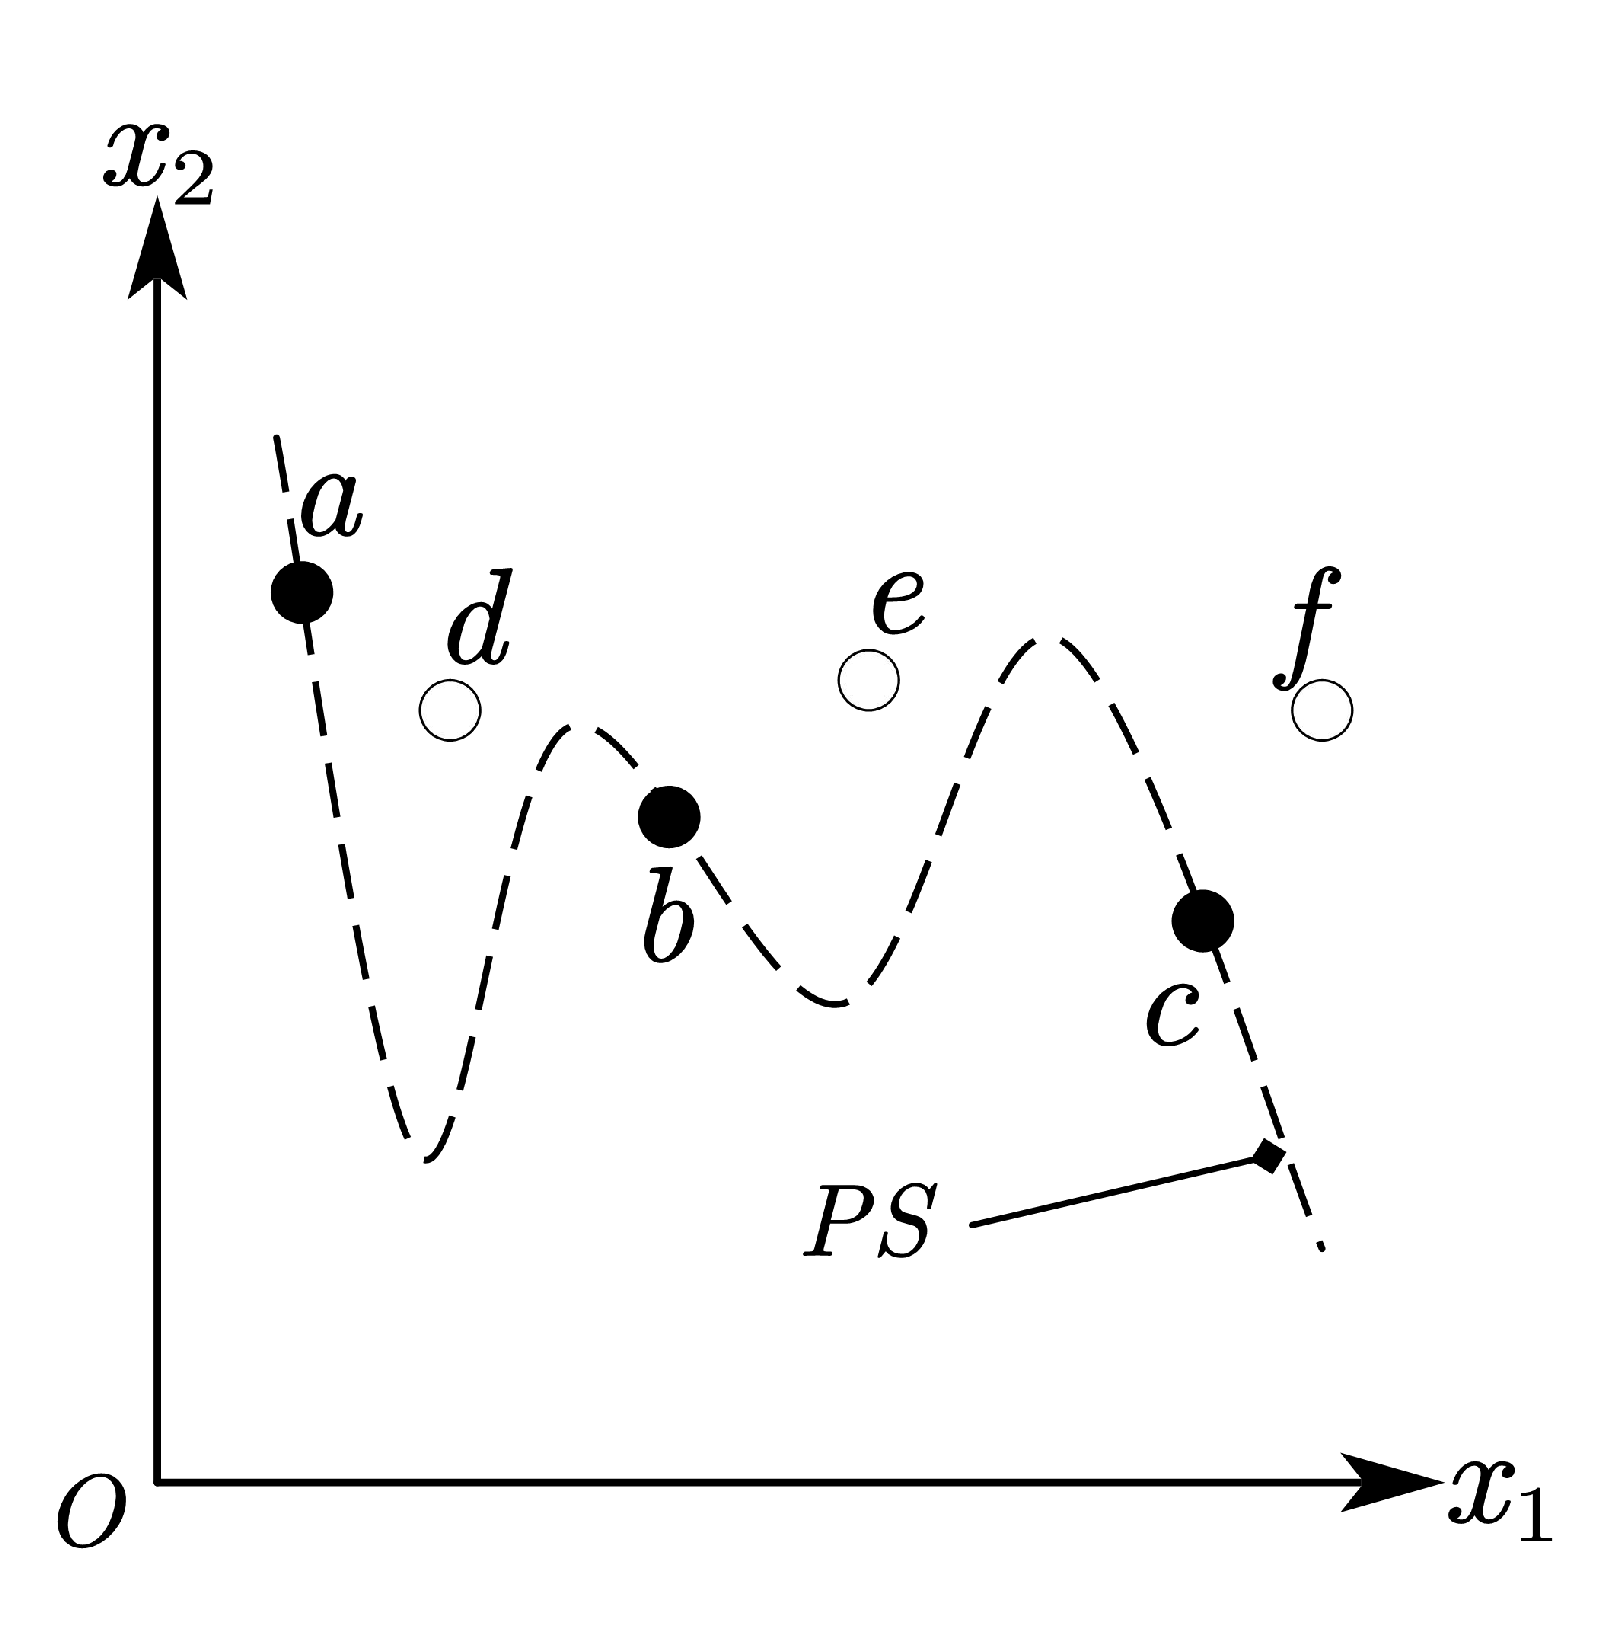
\includegraphics[width=.4\linewidth]{决策空间.pdf}}
    \subfloat[目标空间\label{subfig:目标空间}]{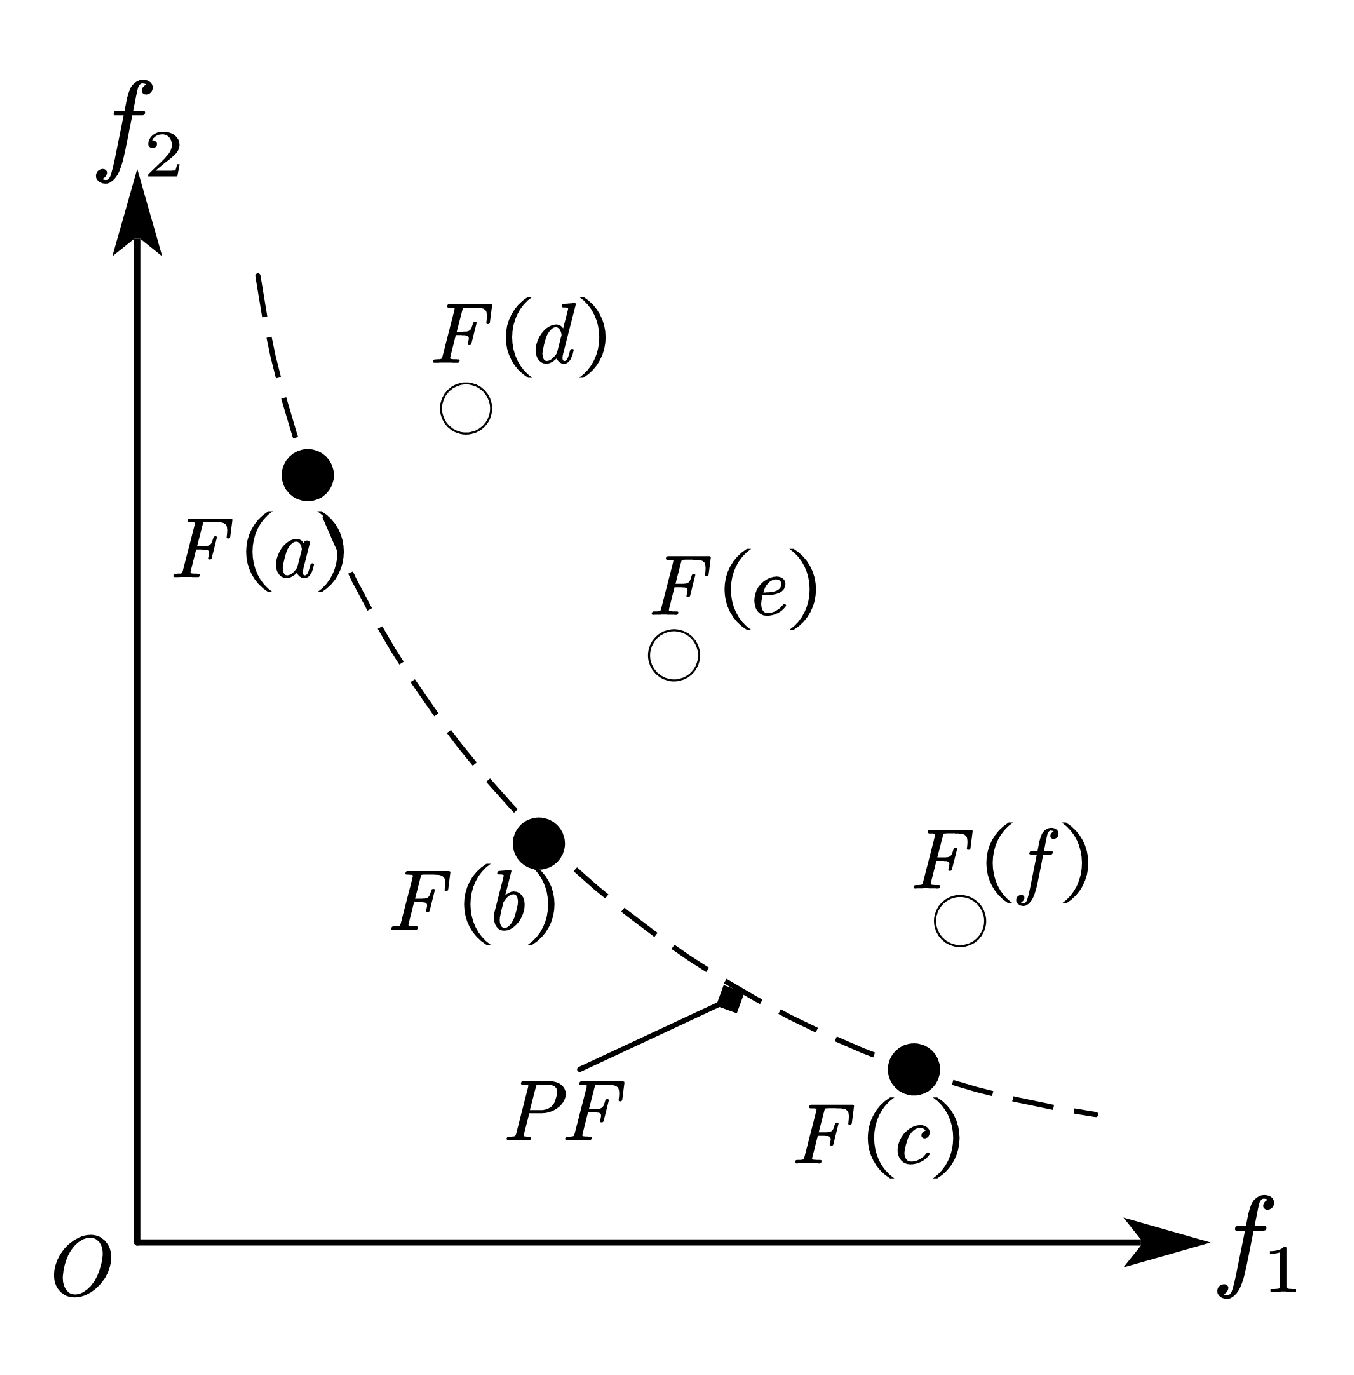
\includegraphics[width=.4\linewidth]{目标空间.pdf}}
    \caption{MOP中相关概念示意图}
    \label{fig:MOP中相关概念示意图}
\end{figure}
\par
设计多目标优化算法时,在目标空间中,还有两个比较重要的概念:理想点(Ideal Point)和边界点(Nadir Point),他们限定了PF的空间范围。
\par
\begin{definition}[理想点(Ideal Point)]
    \label{def:理想点}
    目标空间中,所有可行解$\mathbf{x} \in \Omega$在各个目标上的最小值构成的向量称为理想点(理想目标向量),记作$\mathbf{z}^* = \{ z_1^*, \cdots, z_m^* \}^T$,即
    \begin{align}
        \label{eq:理想点}
        z_i^* = \min_{x \in \Omega} f_i(\mathbf{x}), \ i \in \{ 1, \cdots, m \}.
    \end{align}
\end{definition}
\par
\begin{definition}[边界点(Nadir Point)]
    \label{def:边界点}
    目标空间中,PS中所有可行解$\mathbf{x}$在各个目标上的最大值构成的向量称为边界点(边界目标向量),记作$\mathbf{z}^{nad} = \{ z_1^{nad}, \cdots, z_m^{nad} \}^T$,即
    \begin{align}
        \label{eq:边界点}
        z_i^{nad} = \max_{x \in PS} f_i(\mathbf{x}), \ i \in \{ 1, \cdots, m \}.
    \end{align}
\end{definition}
\par
\begin{figure}[htb]
    \subfloat[2目标MOP\label{subfig:极值点-2D}]{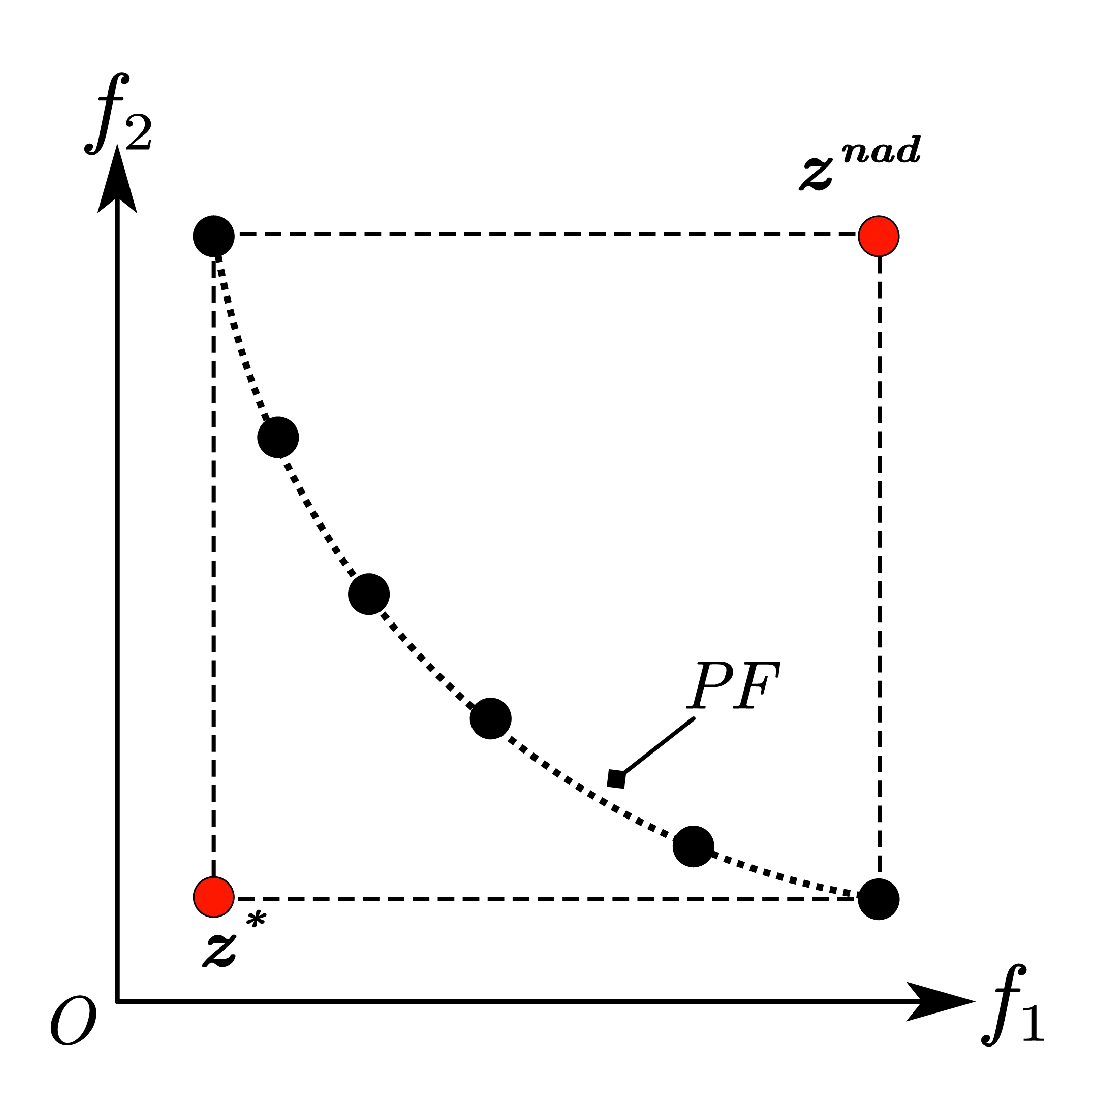
\includegraphics[width=.4\linewidth]{极值点-2D.pdf}}
    \subfloat[3目标MOP\label{subfig:极值点-3D}]{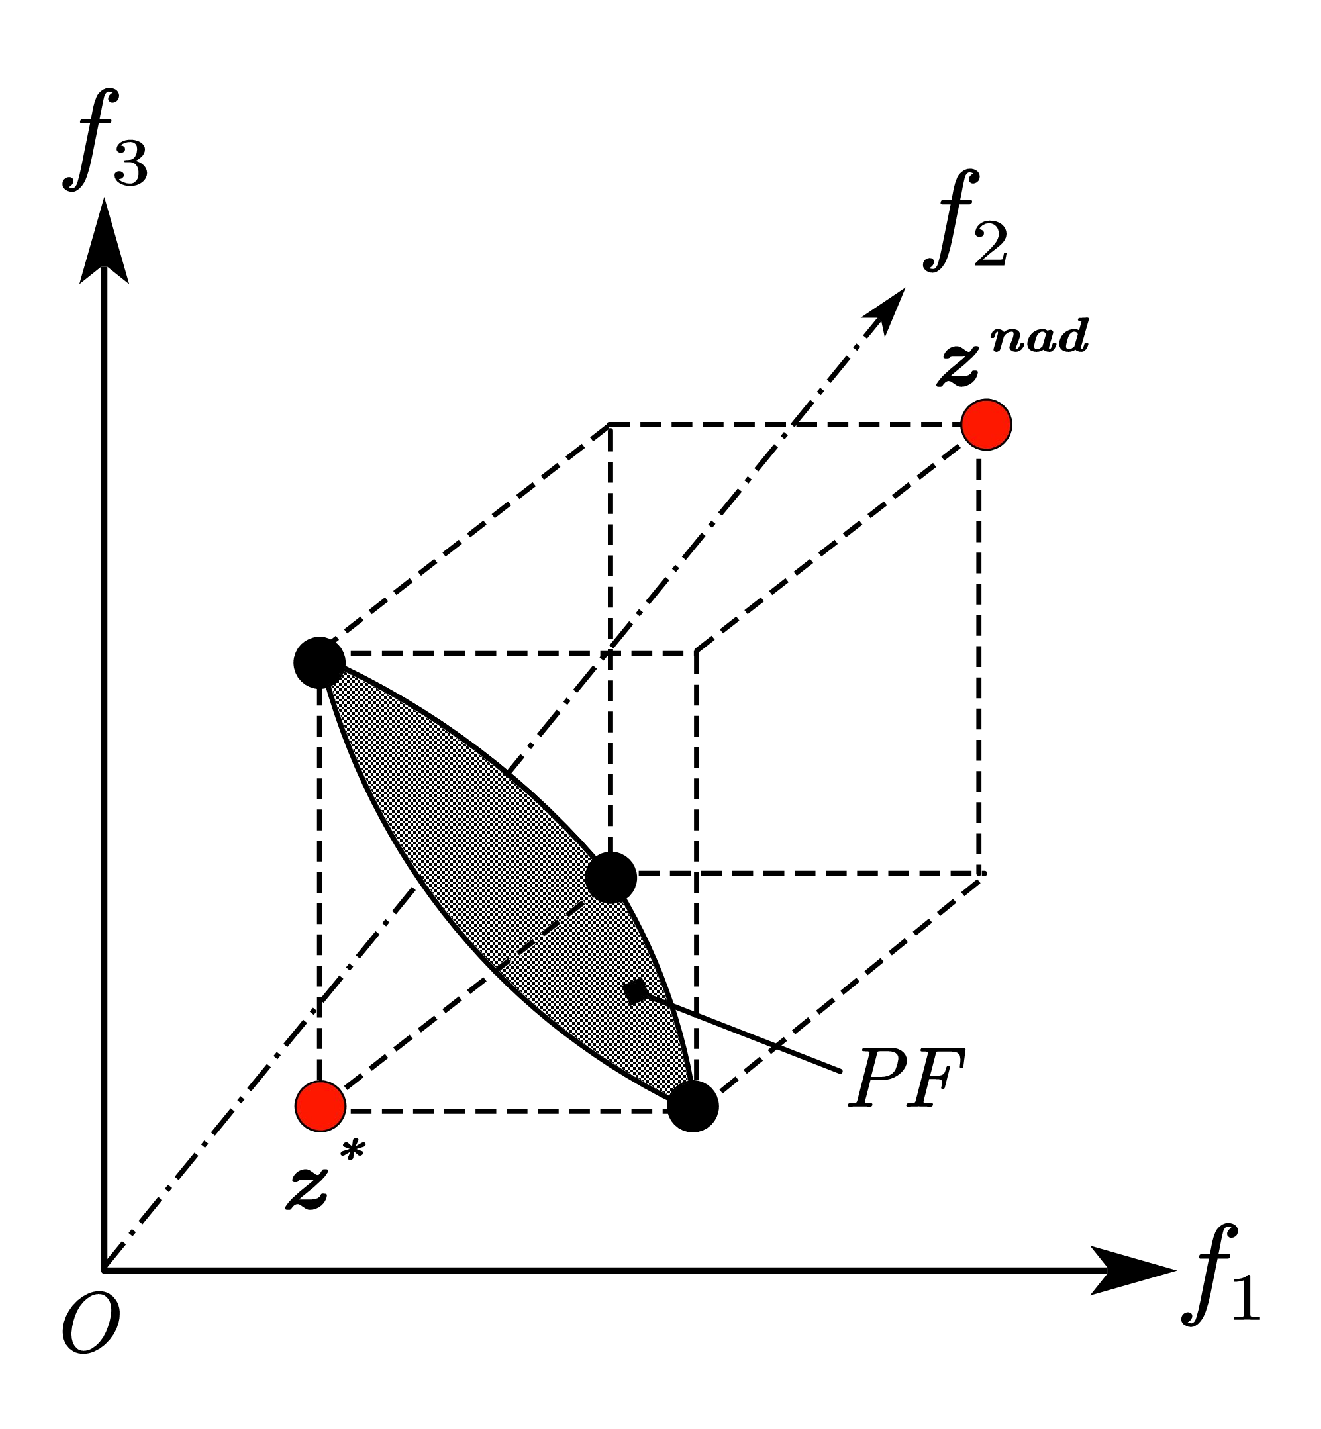
\includegraphics[width=.4\linewidth]{极值点-3D.pdf}}
    \caption{理想点和边界点示意图}
    \label{fig:理想点和边界点示意图}
\end{figure}
\par
如\autoref{fig:理想点和边界点示意图}~中所示,\autoref{subfig:极值点-2D}~和\autoref{subfig:极值点-3D}~分别为两目标和三目标MOP理想点和边界点示意图。由图可以看出,理想点和边界点限定了PF所在区域,分别确定其上下界。

\section{多目标组合优化算法}
\label{sec:背景介绍:多目标组合优化算法}
在大多数MOP中,都需要同时考虑多个互相冲突的目标,通常这些目标难以同时都达到最好的效果,其中一个目标的性能的提升往往会导致问题中的另外一个或多个目标的性能降低。这就需要在优化各个目标时进行权衡,这也致使算法最终求得的解不是惟一的,而是一组互不支配的解(非支配解集)。而这也是进化算法适合求解MOP的原因之一,进化算法正是一种基于群体(多个解)的迭代算法。对于进化算法而言,群体之间的信息遗传(共享)能够促进群体间个体的多元性,并且能够保证群体中的一些优秀信息能被下一代群体继承,进而使得整个群体进化(优化)。由此,本论文基础算法是基于进化算法的,并且,在本节中,首先介绍多目标进化算法的基本框架,然后会对一些多目标组合优化相关的优化技术进行详细介绍。

\subsection{进化算法}
\label{subsec:背景介绍:多目标组合优化算法:进化算法}
进化算法(EA)是一种无需太多问题的先验假设,使用种群循环迭代的方式来有效解决大规模问题的随机全局搜索算法。EA的主要指导思想是基于达尔文的进化论,通过适者生存、优胜劣汰的遗传机制来使得种群在表现出基因多样性的同时相互竞争,从而使得种群进化。EA正是通过模拟自然界物种的行为,在解空间随机的搜索可行解,产生后代种群的同时对种群进行适者生存、优胜劣汰的遗传操作,将高质量的可行解保留,低劣的解淘汰,从而保证算法是往最优解的方向逼近直至收敛。由于EA本身的高适应性和高扩展性的优点,EA可以与现有的启发式算法相组合,被广泛应用于求解各种优化问题。
\par
为了模拟自然界的物种进化,MOEA之中引入了个体、种群、适应度、遗传操作、选择策略等概念:
\begin{itemize}
    \item \textbf{个体:}在实际问题抽象成解空间后,将解编码成能表示其信息的向量(符号串),这个向量(符号串)就是个体。
    \item \textbf{种群:}个体的集合,进化的对象。
    \item \textbf{适应度:}度量个体对于环境的适应程度(个体的质量)。个体的适应度越高,说明该个体的生存能力越强。
    \item \textbf{遗传操作:}一般包括复制(Reproduction)、交叉(Crossover)和变异(Mutation)三种基本形式,是EA的核心部分。在算法中,通过设置三种算子起作用的概率,从而来控制整个群体的进化方向。
    \item \textbf{选择策略:}是从父代中挑选出子代种群的策略,常用的有非支配排序(Non-dominated Sort,NDSort)\cite{srinivas1994muiltiobjective,jensen2003reducing,tang2008fast,mcclymont2012deductive,zhang2014efficient}、拥挤距离(Crowding Distance)\cite{kundu2011multi}、精英保留等策略\cite{deb2002fast}或者混合策略。
\end{itemize}
\par
随着问题的不同,上述MOEA中的部件也会有所不同,我们通常需要根据具体的问题,设计出适用于对应问题的算子。其算法框架如下:
\begin{algorithm}
    \setstretch{1.5}
    \caption{多目标进化算法框架}
    \label{alg:多目标进化算法框架}
    \BlankLine
    \KwIn{ \\
        \hspace{1em} $\mathbf{MOP}$:多目标优化问题 \\
        \hspace{1em} $\mathbf{params}$:种群参数 \\
        \hspace{1em} $\mathbf{stop}$:终止条件
    }
    \KwOut{$\mathcal{PS}$}
    $\mathcal{P} \xleftarrow[]{\text{初始化}} \mathbf{MOP},\mathbf{params}$ \;
    \While{not $\mathbf{stop}$}{
        $\mathcal{P}^{'} \xleftarrow[]{\text{遗传操作}} \mathcal{P} $ \;
        $\mathcal{P}_{new} \leftarrow \mathcal{P} \bigcup \mathcal{P}^{'} $\;
        $fitness \xleftarrow[]{\text{适应度评价}} \mathcal{P}_{new} $ \;
        $\mathcal{P} \xleftarrow[fitness]{\text{选择策略}} \mathcal{P}_{new} $ \;
    }
    $\mathcal{PS} \xleftarrow[]{NDSort} \mathcal{P} $ \;
    \textbf{return } $\mathcal{PS}$ \;
\end{algorithm}
\par
\begin{figure}[htb]
    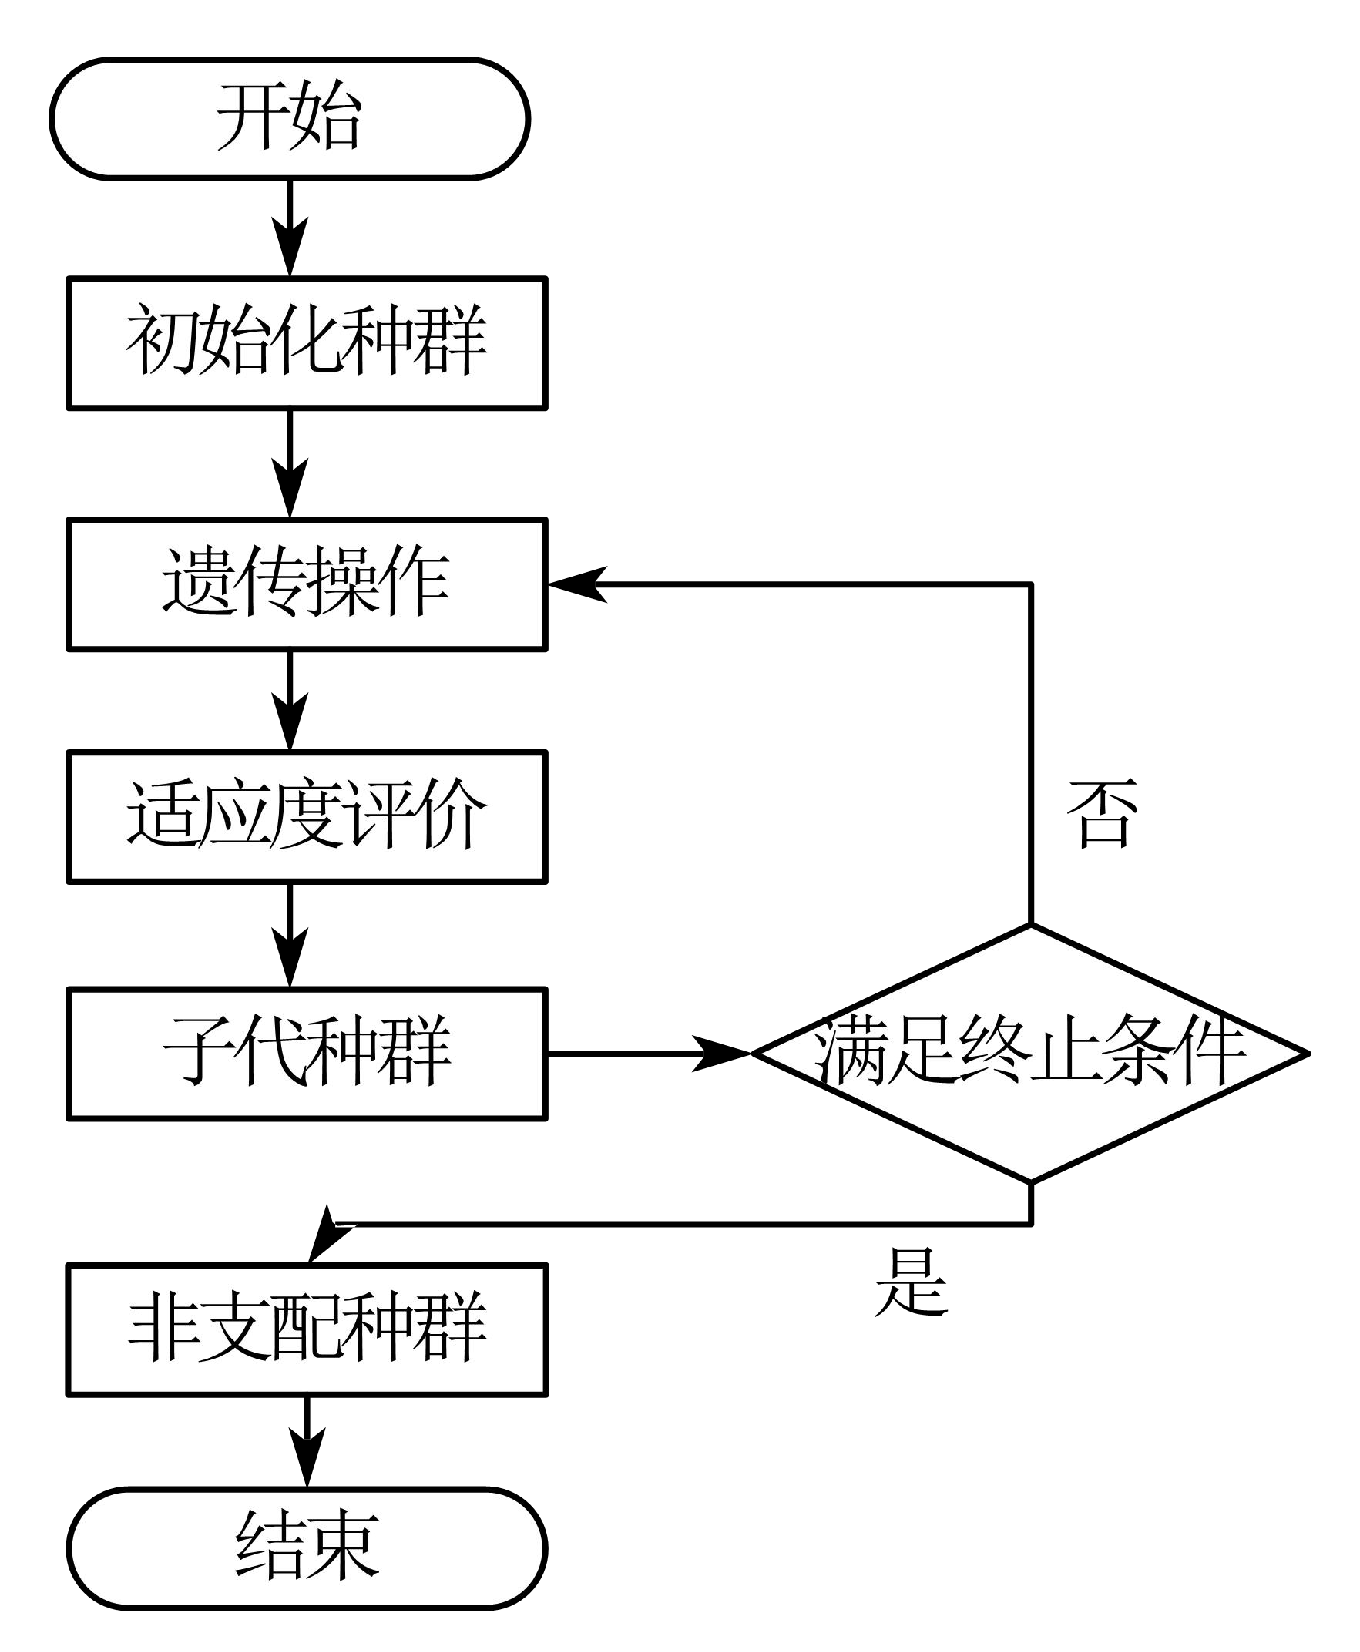
\includegraphics[width=.5\linewidth]{多目标进化算法流程.pdf}
    \caption{多目标进化算法流程图}
    \label{fig:多目标进化算法流程图}
\end{figure}
\par
算法~\ref{alg:多目标进化算法框架}~是多目标进化算法的基本框架,与\autoref{fig:多目标进化算法流程图}~展示的多目标进化算法流程图相对应。在算法中,首先随机初始化一个种群$\mathcal{P}$,$\mathcal{P}$中的个体即为问题的初始解,个体是根据MOP而设计的向量或符号串,种群规模根据$\mathbf{params}$而设置。接下来就是迭代过程,模拟的是种群的进化。然后对种群$\mathcal{P}$进行遗传操作(对于不同的问题,遗传操作也不尽相同。组合优化通常采用局部搜索的方式产生新的个体,局部搜索算子也需要单独设计)产生新的种群$\mathcal{P}^{'}$,接着将父代种群和新产生的种群混合,获取它们所有个体的评价值,然后根据评价值和选择策略选出子代种群(选择策略通常采用的是精英选择策略,是算法中至关重要的一步,它需要确保种群能够向着好的方向进化,即向PF逼近,同时还需要兼顾多样性和收敛性这两个关键指标)。最后在末代的时候,采用非支配排序的方式,从种群$\mathcal{P}$中选出非支配种群$\mathcal{PS}$。
\par
由算法~\ref{alg:多目标进化算法框架}~和\autoref{fig:多目标进化算法流程图}~展示的多目标进化算法的工作流程,可以清晰的知道,如何产生和挑选子代种群是我们在设计算法时需要关注的对象。但是,没有在算法~\ref{alg:多目标进化算法框架}~和\autoref{fig:多目标进化算法流程图}~中体现的细节,也是本文研究的重点。比如:
\begin{itemize}
    \item 设计容易表达问题的个体
    \item 算法终止的条件
    \item 局部搜索算法(产生新个体的方法,设计问题的邻域结构)
\end{itemize}

\subsection{基于分解的多目标进化算法}
\label{subsec:背景介绍:多目标组合优化算法:基于分解的多目标进化算法}
1985年,Fourman和Schaffer等人在解决多目标优化问题时提出多目标进化算法\cite{fourman1985compaction,schaffer1985multiple},经由多年的研究发展,已经衍生出各种各样的多目标进化算法,按照不同的策略大致可以归纳为三类算法框架:基于支配的(Domination-based)、基于分解的(Decomposition-based)和基于指标的(Indicator-based)多目标进化算法。尽管基于支配的和基于指标的多目标进化算法框架仍然被广泛的使用,但是由于各自算法机制的原因,导致他们在很多方面有着的局限性。基于支配的多目标进化算法框架的缺陷在于它不适用于超多目标(优化目标数$m > 3$)的优化问题,在超多目标优化问题的解集中,几乎所有的解之间都是非支配的,这使得非支配排序算法几乎失效,导致算法中的选择策略不能为种群进化提供有效的指导,最终导致算法不能向PF逼近,不能起到优化的作用\cite{ishibuchi2008behavior,giagkiozis2015methods}。同样,基于指标的多目标进化算法框架的其中一个局限性是,它依赖于指标的计算,然而大多数指标的计算复杂度会随着问题目标的数量呈指数级增长,这导致算法难以在有效时间内使用,如基于超体积指标的多目标进化算法,其计算复杂度随目标数呈指数上升,即使目前有很多能够降低复杂度的近似方法,也不能满足多目标优化问题的效率需求。
\par
近年来,在对多目标进化算法的研究中,基于分解的多目标进化算法越来越受到研究者们的关注,其核心思想是通过分解的方式,将一个多目标优化问题分解为一组单目标的子问题,然后使用优化算法对这些单目标子问题同时进行优化,最后将这些单目标子问题的解组合成一个多目标优化问题的解集。在早期,分解的思想就在解决多目标优化问题的几个启发式算法中得到了一定程度上的应用\cite{ishibuchi1998multi,jin2001adapting,jaszkiewicz2002performance,paquete2003two,hughes2003multiple}。2007年,Zhang等人结合分解的思想,系统的提出了基于分解的多目标进化算法(MOEA/D)\cite{zhang2007moea},成为了最热门的基于分解的多目标进化算法之一。近来更是涌现出各种基于MOEA/D的算法框架,被用来解决各种各样的多目标优化问题\cite{ke2013moea,ke2014hybridization}。
\par
在MOEA/D中,它把一个多目标优化问题根据一组权重向量分解成多个单目标子问题,然后根据各个子问题之间的联系形成邻居关系,然后利用邻居子问题之间的信息对所有子问题进行优化。对于一个具有$m$个目标的MOP,将其分解成$k$个子问题,首先需要定义$k$个均匀的权重向量,其中一个权重向量$\boldsymbol{\lambda}$为:
\begin{align}
    \label{eq:背景介绍:权重向量}
    \boldsymbol{\lambda} = (\lambda_1, \cdots. \lambda_m)^T, \quad \forall \lambda_i \geq 0 , \quad \sum_{i=1}^m \lambda_i = 1. 
\end{align}
然后,针对不同类型的问题,可以使用不同的分解方法,下面将介绍三种常用的分解方法(聚合函数):
\par
\begin{enumerate}
    \item \textbf{加权和法(Weight Sum,WS):}WS是一种常用的线性多目标优化问题的聚合方法\cite{hillermeier2001nonlinear},它的目标函数聚合形式为可定义为:
    \begin{align}
        \label{eq:WS}
        minimize \quad & g^{ws}(\mathbf{x} \ | \ \boldsymbol{\lambda}) = \sum_{i=1}^m \lambda_i f_i(\mathbf{x}), \\
        subject \ \ to \quad & \mathbf{x} \in \Omega. \notag
    \end{align}
    其中$\mathbf{x}$是决策向量,$\boldsymbol{\lambda}$为权重向量。
    \begin{figure}[htb]
        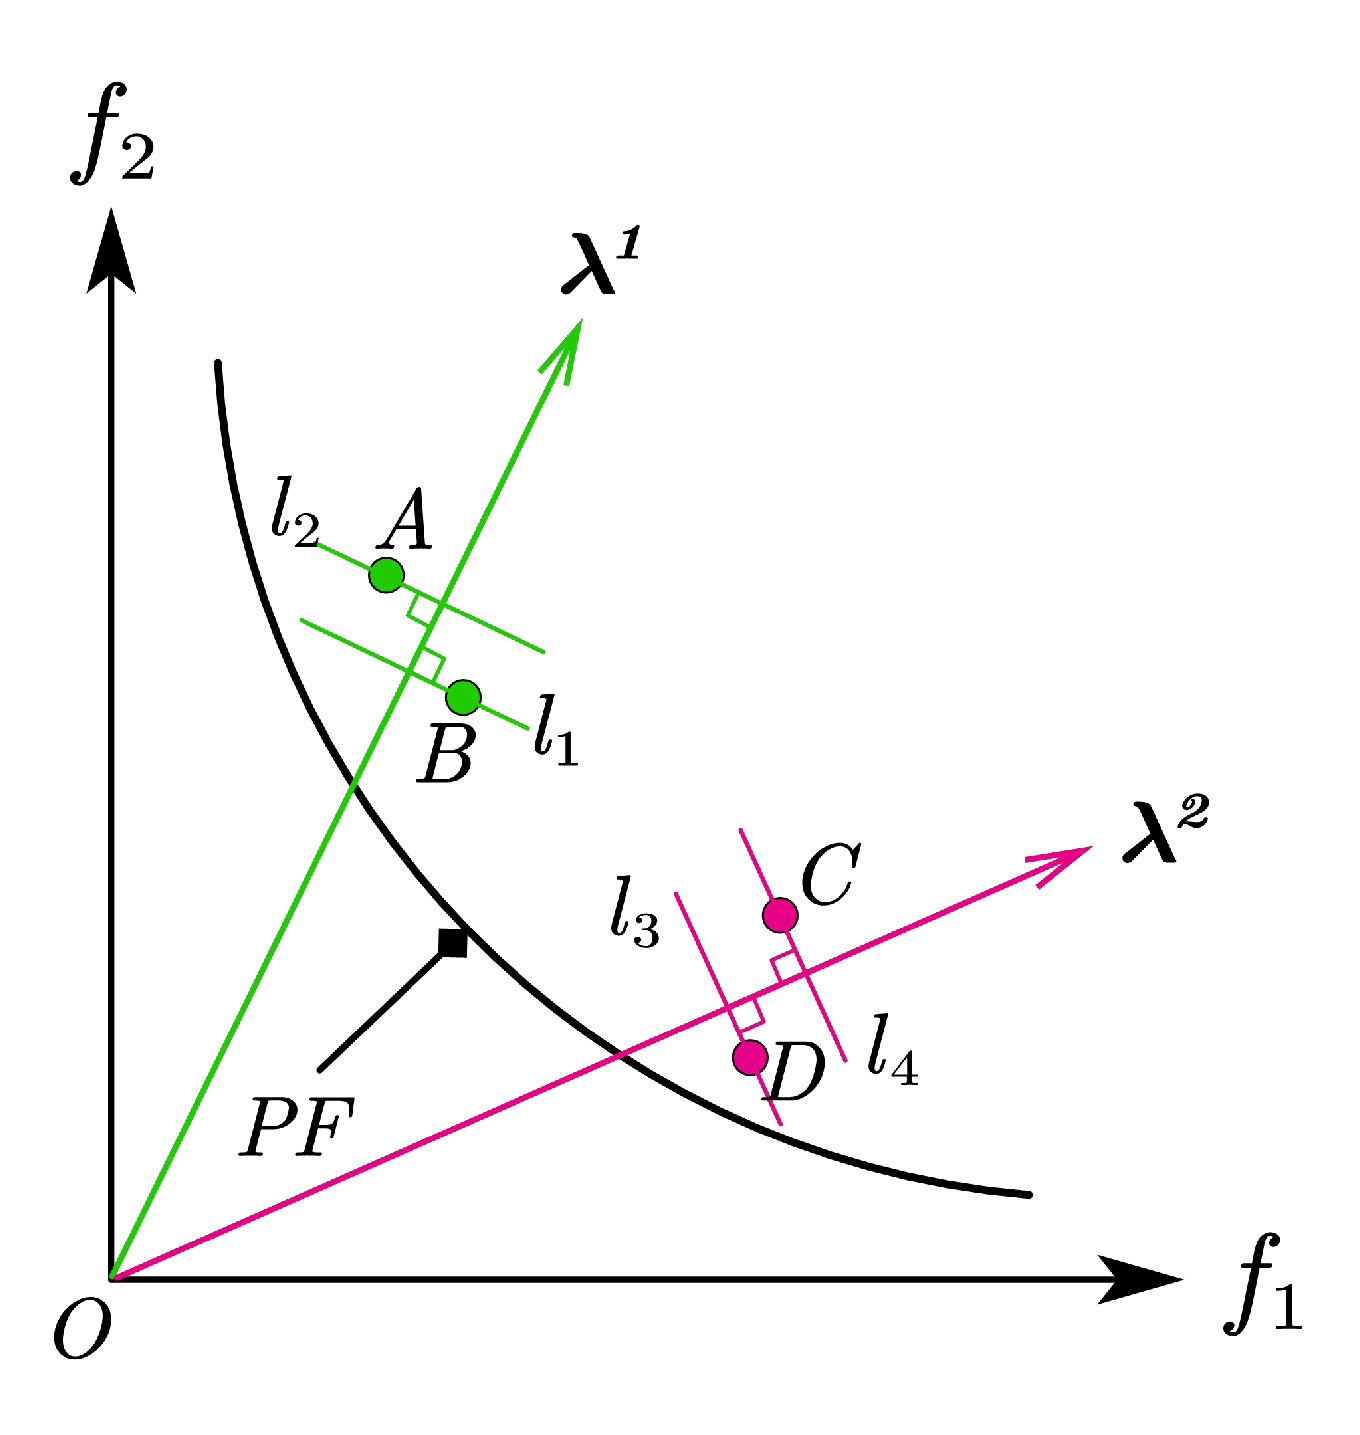
\includegraphics[width=.4\linewidth]{WS等高线.pdf}
        \caption[加权和法(WS)等高线示意图]{加权和法(WS)等高线示意图 \\ $\boldsymbol{\lambda^1}$和$\boldsymbol{\lambda^2}$分别为两个子问题的权重向量,$l_1, l_2, l_3, l_4$分别为对应子问题的等高线}
        \label{fig:WS等高线示意图}
    \end{figure}
    \par
    \autoref{fig:WS等高线示意图}~展示的是一个二目标优化问题使用加权和法的等高线示意图。容易看出,加权和法的等高线是一簇与权重向量$\boldsymbol{\lambda}$垂直的平行直线。个体在权重向量上的投影长度即为该个体在所属$\boldsymbol{\lambda}$上的子问题的聚合值。在\autoref{fig:WS等高线示意图}~中,个体A和B是互不支配的,但是,在$\boldsymbol{\lambda^1}$所属子问题上用加权和法后,个体B要优于个体A,因为个体B在$\boldsymbol{\lambda^1}$上的投影长度要比个体A短。同理,个体D优于个体C。
    \item \textbf{切比雪夫法(Tchebycheff,TCH):}TCH是一种非线性多目标聚合方法\cite{jaszkiewicz2002performance},它的目标函数聚合形式可定义为:
    \begin{align}
        \label{eq:TCH}
        minimize \quad & g^{tch}(\mathbf{x} \ | \ \boldsymbol{\lambda},\mathbf{z}^*) = \max_{1 \leq i \leq m} \lambda_i | f_i(\mathbf{x}) - z^*_i |, \\
        subject \ \ to \quad & \mathbf{x} \in \Omega. \notag
    \end{align}
    其中$\mathbf{x}$是决策向量,$\boldsymbol{\lambda}$为权重向量,$\mathbf{z}^*$为理想点(\autoref{def:理想点})。
    \par
    \begin{figure}[htb]
        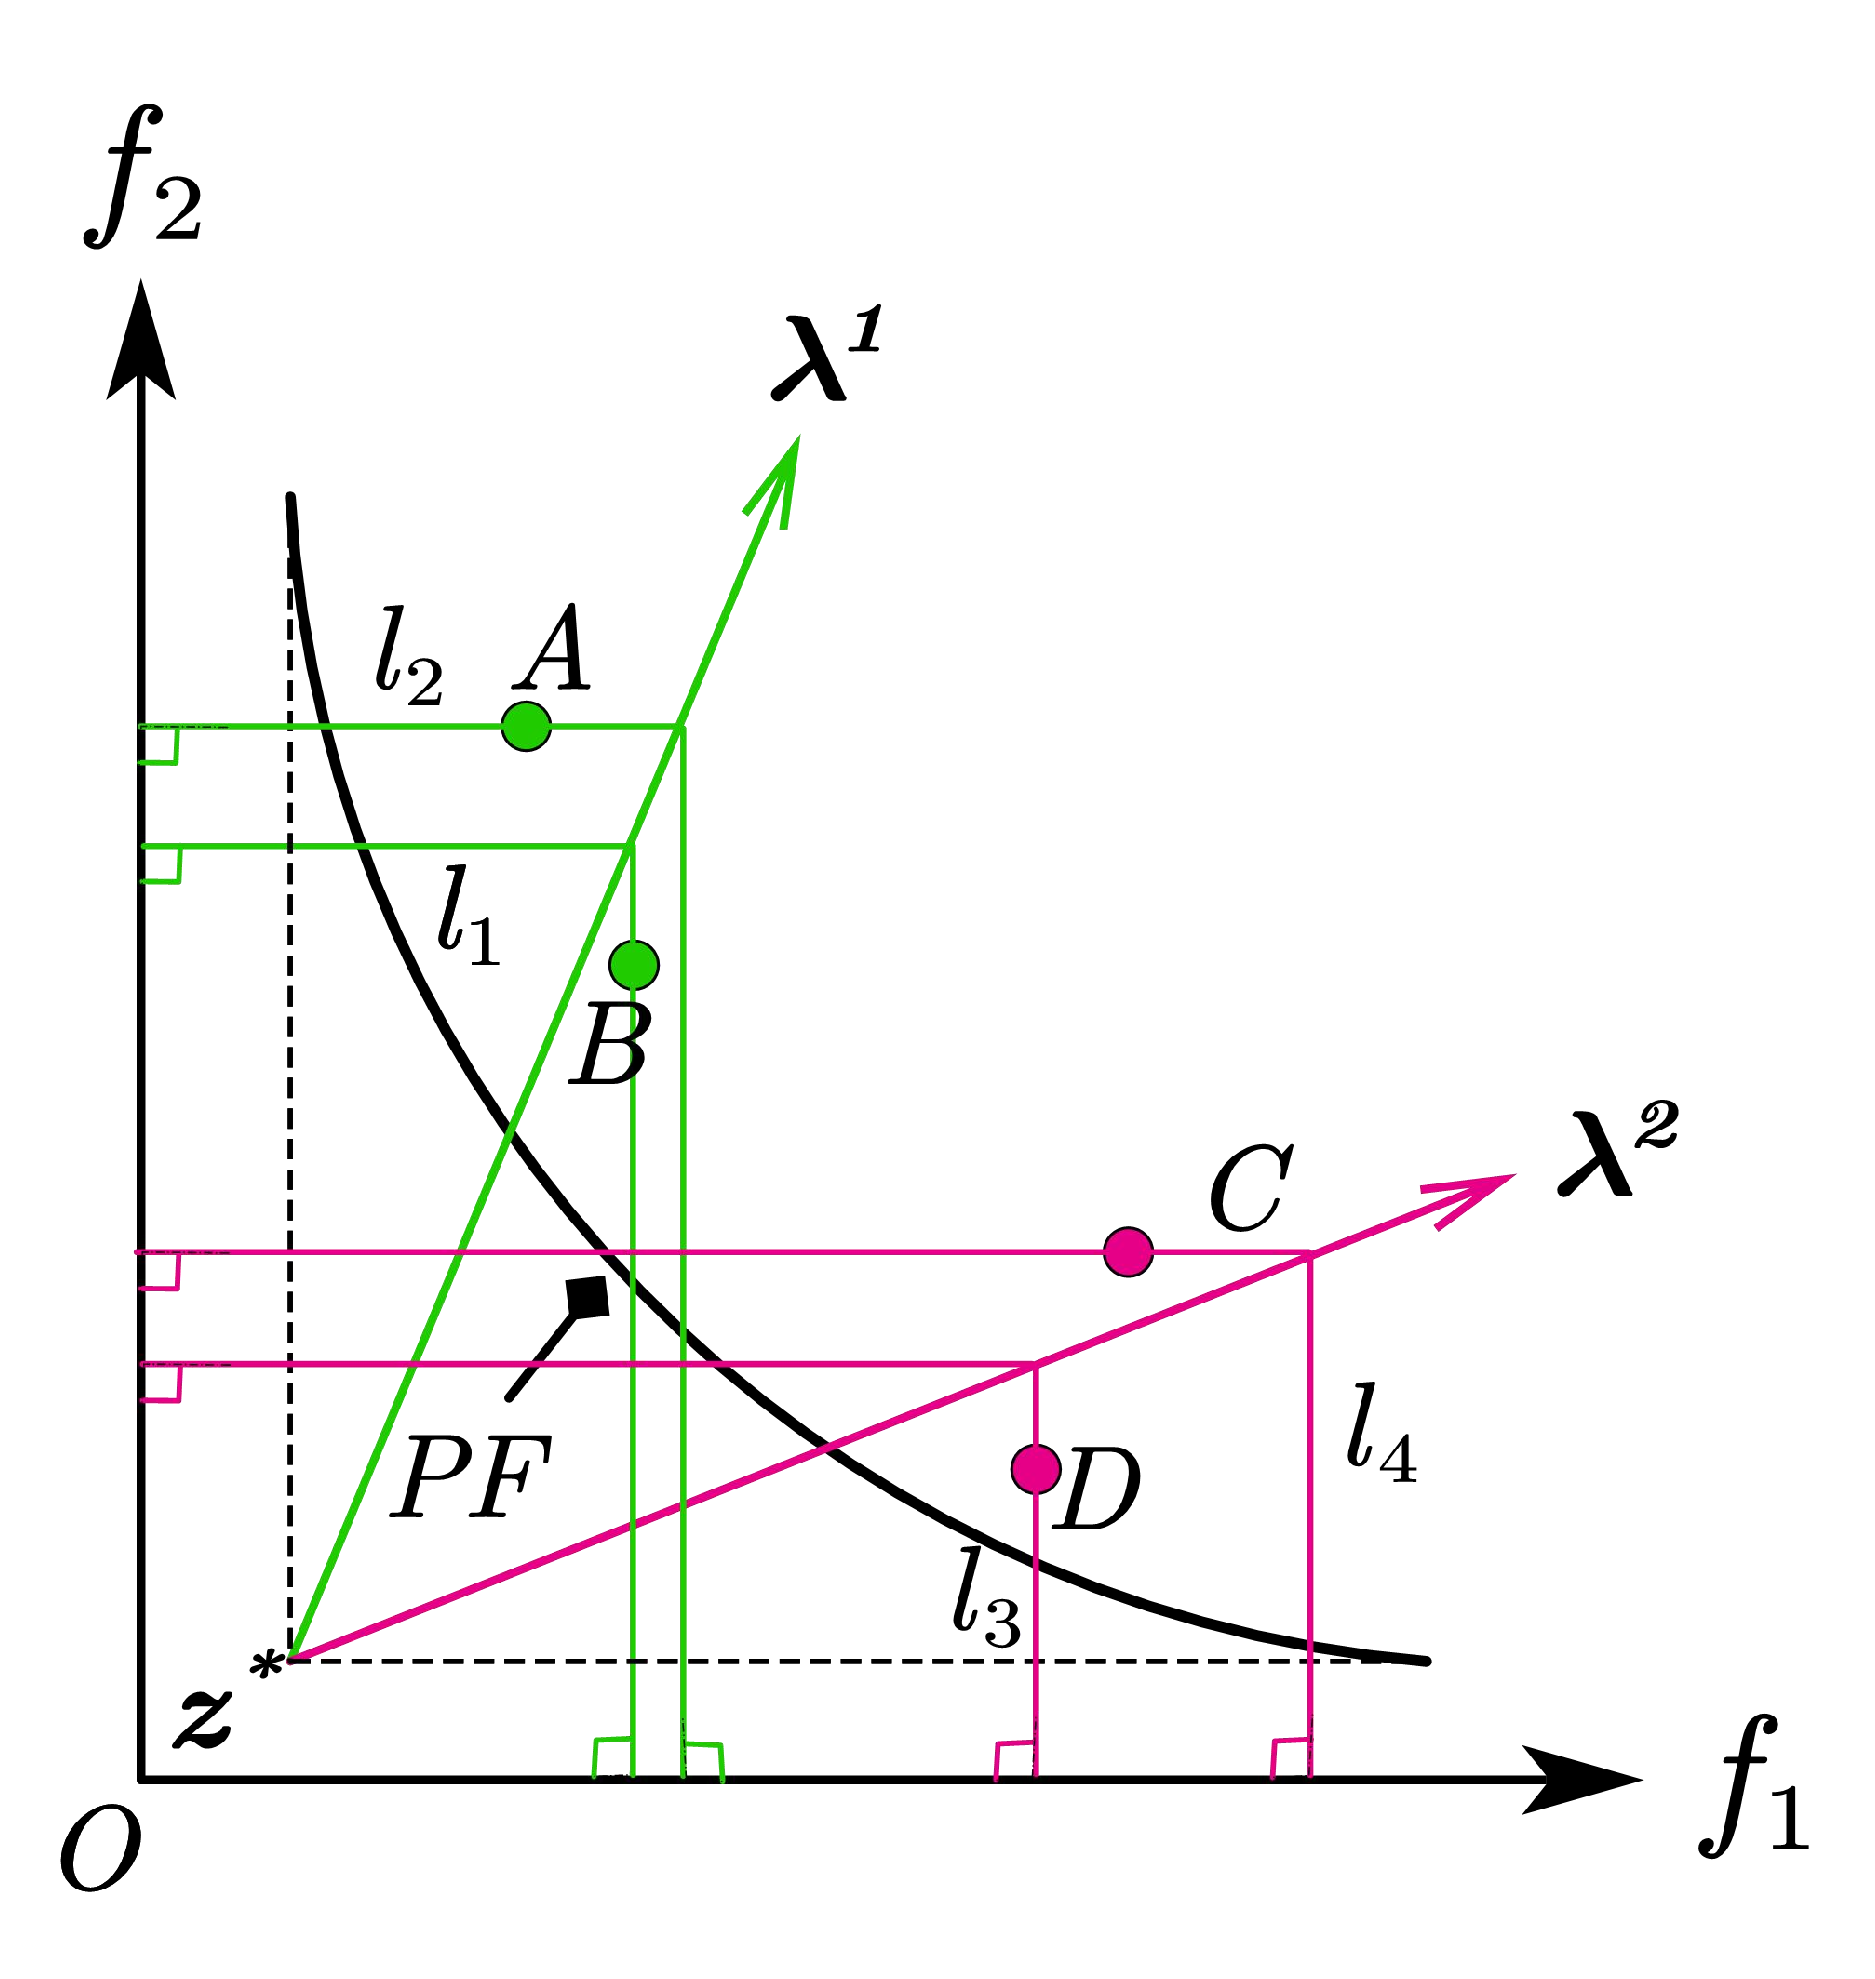
\includegraphics[width=.4\linewidth]{TCH等高线.pdf}
        \caption[切比雪夫法(TCH)等高线示意图]{切比雪夫法(TCH)等高线示意图 \\ $\boldsymbol{\lambda^1}$和$\boldsymbol{\lambda^2}$分别为两个子问题的权重向量,$l_1, l_2, l_3, l_4$分别为对应子问题的等高线}
        \label{fig:TCH等高线示意图}
    \end{figure}
    \par
    \autoref{fig:TCH等高线示意图}~展示的是一个二目标优化问题使用切比雪夫法的等高线示意图。从\autoref{fig:TCH等高线示意图}~中可以看出,对于$\boldsymbol{\lambda^1}$所属子问题,个体B优于个体A,因为个体B的切比雪夫聚合值要优于个体A。同理,个体D优于个体C。从图中还可以分析出,在连续PF时,用TCH分解方法得到的子问题的最优解是权重向量与PF面的交点。在非连续PF时,由于权重向量可能和PF面没有交点,所属不同权重向量的子问题可能具有相同的最优解。相比于加权和法,TCH分解方法的等高线沿着权重向量呈直角锯齿形,因此,用TCH方法得到的子问题具有更小的收敛区域(搜索空间),这在处理高维问题时,TCH分解方法能够很好的限制收敛区域,因此能够很好的保证种群的收敛性。
    \item \textbf{基于惩罚的边界交叉法(Penalty-based Boundary Intersection,PBI):}PBI是由Zhang等人于2007年提出的一种分解方法\cite{zhang2007moea},它的目标函数聚合形式为:
    \begin{align}
        \label{eq:PBI}
        minimize \quad & g^{pbi}(\mathbf{x} \ | \ \boldsymbol{\lambda},\mathbf{z}^*) = d_1 + \theta d_2, \\
        & d_1 = \frac{\| (\mathbf{z}^* - F(\mathbf{x}))^T \boldsymbol{\lambda} \Vert }{ \|  \boldsymbol{\lambda} \Vert }, \notag\\
        & d_2 = \| F(\mathbf{x}) - (\mathbf{z}^* - d_1 \boldsymbol{\lambda}) \Vert, \notag \\
        subject \ \ to \quad & \mathbf{x} \in \Omega. \notag
    \end{align}
    其中$\mathbf{x}$是决策向量,$\boldsymbol{\lambda}$为权重向量,$\mathbf{z}^*$为理想点(\autoref{def:理想点}),$d_1$表示目标向量$F(\mathbf{x})$到权重向量$\boldsymbol{\lambda}$的投影长度,$d_2$表示目标向量$F(\mathbf{x})$到权重向量$\boldsymbol{\lambda}$的垂直距离,$\theta$为惩罚因子,用于调节$d_1$和$d_2$之间的平衡,控制种群的分布性和收敛性。
    \par
    \begin{figure}[htb]
        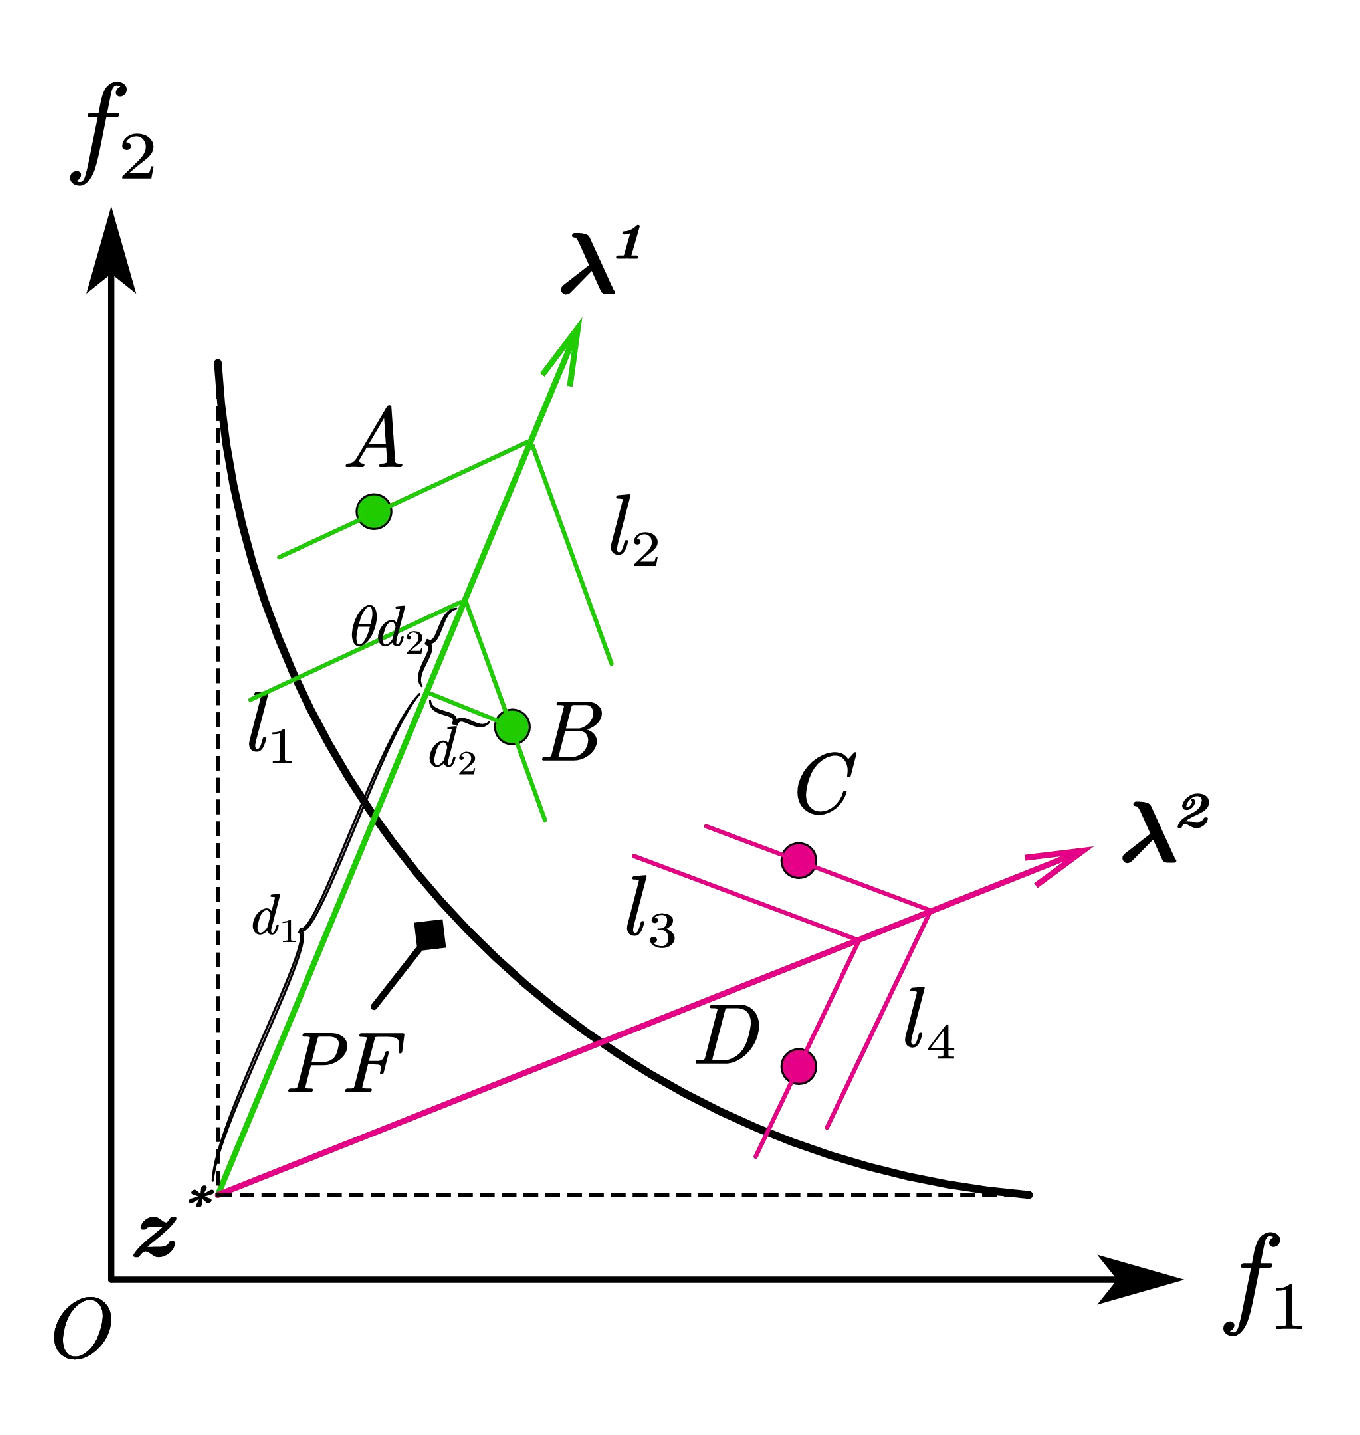
\includegraphics[width=.4\linewidth]{PBI等高线.pdf}
        \caption[基于惩罚的边界交叉法(PBI)等高线示意图]{基于惩罚的边界交叉法(PBI)等高线示意图 \\ $\boldsymbol{\lambda^1}$和$\boldsymbol{\lambda^2}$分别为两个子问题的权重向量,$l_1, l_2, l_3, l_4$分别为对应子问题的等高线}
        \label{fig:PBI等高线示意图}
    \end{figure}
    \par
    \autoref{fig:PBI等高线示意图}~展示的是一个二目标优化问题使用基于惩罚的边界交叉法的等高线示意图。在图中,$d_1$是个体B到权重向量$\boldsymbol{\lambda^1}$的投影长度,$d_2$是个体B到权重向量$\boldsymbol{\lambda^1}$的垂直距离,$d_1+\theta d_2$即为PBI聚合值。显然,对于$\boldsymbol{\lambda^1}$所属子问题,个体B的PBI聚合值要优于个体A,即个体B优于个体A。同理,个体D优于个体C。通过\autoref{eq:PBI}~和\autoref{fig:PBI等高线示意图}~可以知道,PBI能够通过调节$\theta$参数来控制$d_1$和$d_2$之间的平衡,从而控制种群的分布性和收敛性。由于能够控制分布性和收敛性之间的平衡这一特点,PBI分解方法在处理高维目标(超多目标)问题时具有很大的优势。但是,参数$\theta$的设置也影响着算法的性能表现,这同时也成为PBI分解方法的缺点之一。
\end{enumerate}
\par
MOEA/D算法的核心思想是将MOP分解成一系列单目标子问题或者多个多目标子问题,然后利用这些子问题的邻域相似度,通过协作的方式来同时优化所有子问题,从而向PF逼近。通常子问题有权重向量通过聚合函数确定,这些子问题之间的邻域关系是通过各个子问题的权重向量之间的相似度(欧式距离)来度量的。与其他的多目标进化算法不同的是,MOEA/D算法注重从当前子问题的邻域子问题中选择父个体,通过遗传算子(交叉、变异算子)来生成新个体,并且按照一定的策略来更新邻域中的种群。因此,一个优秀的基于邻域的优化策略能够确保MOEA/D算法的搜索效率。在算法的迭代进化过程中,一旦搜索到针对某个子问题的高质量解,这个解的优质信息就会迅速的被邻域内的其他个体继承,从而加快整个种群进化(收敛)的速度。下面是MOEA/D算法的一个基本框架流程:
\begin{algorithm}[ht]
    \caption{MOEA/D算法框架}
    \label{alg:MOEA/D算法框架}
    \BlankLine
    \KwIn{ \\
        \hspace{1em} $\mathbf{MOP}$:多目标优化问题 \\
        \hspace{1em} $\mathbf{N}$:子问题个数 \\
        \hspace{1em} $\mathbf{T}$:邻域大小 \\
        \hspace{1em} $\boldsymbol{\lambda}$:一组均匀分布的权重向量 $\{ \boldsymbol{\lambda^1}, \cdots, \boldsymbol{\lambda^N} \}$\\
        \hspace{1em} $\mathbf{stop}$:终止条件
    }
    \KwOut{$\mathcal{EP}$:外部集(精英种群)}
    $\mathcal{SP} = \{ SP_1, \cdots, SP_N \} \xleftarrow[\mathbf{N}]{\boldsymbol{\lambda}} \mathbf{MOP}$ \;
    $\mathbf{B}(i) = \{ i_1, \cdots, i_T \}, i \in \{ 1, \cdots, N \}$,其中$\{ \boldsymbol{\lambda}^{i_1}, \cdots, \boldsymbol{\lambda}^{i_T} \}$是最接近$\boldsymbol{\lambda}^i$的$\mathbf{T}$个权重向量 \;
    $\mathcal{P} \xleftarrow[]{\mathbf{N}} $随机生成大小为$\mathbf{N}$的初始种群 \;
    $\mathbf{z}^* \leftarrow $通过\autoref{eq:理想点}更新理想点 \;
    \While{not $\mathbf{stop}$}{
        \For{$i = \{1, \cdots, \mathbf{N}\} $}{
            $\mathbf{x}^{'} \xleftarrow[]{\text{遗传算子}}$ 由$SP_i$的邻居$\mathbf{B}(i)$确定$\mathcal{P}$中的两个个体 \;
            $\mathbf{z}^* \leftarrow$ 用$F(\mathbf{x}^{'})$更新理想点 \;
            通过聚合函数(式\ref{eq:WS},\ref{eq:TCH},\ref{eq:PBI}),用$\mathbf{x}^{'}$更新$SP_i$的邻居解 \;
            $\mathcal{EP} \leftarrow$ 用$F(\mathbf{x}^{'})$更新外部集 \;
        }
    }
    \textbf{return } $\mathcal{EP}$ \;
\end{algorithm}
\par
算法~\ref{alg:MOEA/D算法框架}~可以分为三个阶段:初始化、遗传生成和更新阶段。在初始化阶段,首先将MOP通过权重向量分解成$\mathbf{N}$个子问题$\mathcal{SP} = \{ SP_1, \cdots, SP_N \}$,并且初始化每个子问题的邻居,然后随机生成初始种群$\mathcal{P}$,并得到理想点$\mathbf{z}^*$。在遗传生成阶段主要是从邻居中选出父代个体,然后通过遗传操作来生成子代个体$\mathbf{x}^{'}$。最后的更新阶段就是用生成的子代个体$\mathbf{x}^{'}$来更新邻居解、理想点和外部集。应该注意的是,算法中邻域的大小和替换个体的次数会对种群的分布性和收敛性产生影响。并且在更新阶段,外部集$\mathcal{EP}$中保存着所有被搜索到的非支配解,为了节省资源,可以用一些已有的密度估计方法来控制外部集$\mathcal{EP}$的大小。

\section{局部搜索}
\label{sec:背景介绍:局部搜索}
搜索算法是有目的的穷举一个问题解空间中部分或者所有的可能情况,直到搜索到问题的解的一种方法,实际上是根据初始条件和扩展规则构造一颗解答树并寻找符合目标状态节点的过程。从宏观上看,所有的搜索算法都可以划分为两个部分:控制结构(扩展点的方式)和生成系统(扩展节点),而大多数的算法优化和改进都主要是通过修改控制结构来完成的。
\par
在全局搜索(Global Search,GS)中,需要将所有搜索到的路径都记录下来,直到搜索到最优解(满意解),其中,到达目标状态的搜索路径就是问题的解。但是,在大多数问题中,绝大多数的的搜索路径与最终目标状态并不是紧密相关的。因此,没有必要将所有搜索到的路径都记录下来,只需要关键路径即可,这样能够节省大量的空间和时间。与GS记录所有搜索路径相对,只维护当前目标状态和记录部分关键搜索路径的搜索算法就是局部搜索算法(Local Search,LS)。当问题的状态空间(决策空间)很大时,全局搜索算法就不适用了,其找到最优解所需的时间和空间都将成指数形式的增长,因此,设计效率高的局部搜索算法也是本文研究的重点。并且,本文主要的研究载体是多目标组合优化问题,这类问题的决策空间是离散的,并且十分巨大,导致往常用的遗传算子(交叉、变异等)生成新个体的效率低下。因此,应对这类问题,局部搜索算子就成了算法中必不可缺的一部分。

\subsection{基本概念}
\label{subsec:背景介绍:局部搜索:基本概念}
对于一个组合优化问题,局部搜索算法就是在该问题的候选解空间(邻域结构)上进行搜索,其搜索过程是从选择初始的候选解开始,然后在当前候选解的邻域结构中进行搜索,如此迭代直到找到一个满意的解或者搜索到了局部搜索算法的终止条件。在搜索过程中,每次对候选解是否被选择的决策仅基于有限的局部信息,并且算法中的决策和最开始的初始化可以是随机的。因此,基于以上局部搜索算法过程,可以给定以下定义\cite{blum2003metaheuristics}:
\begin{definition}
    \label{def:CO}
    给定一个最小化CO问题$P = (\mathcal{S}, f)$,变量$\mathbf{x}=\{ x_1, \cdots, x_n \} \in \mathcal{X}$,$\mathcal{X}$是离散有限(可数无限)变量集,其决策域为$\mathcal{D} = \{ D_1, \cdots, D_n \}$,约束域为$\mathcal{C}$,则有
    \begin{align}
        \label{eq:CO}
        minimize \quad & f: D_1 \times \cdots \times D_n \rightarrow \mathbb{R}^+, \\
        s.t. \quad & \mathcal{C}. \notag
    \end{align}
    则所有可能的可行解可表示为:
    \begin{align}
        \label{eq:可行解}
       \mathcal{S} = & \{ s = \{ (x_1, v_1), \cdots, (x_n, v_n) \} \}, \\
        s.t. \quad & v_i \in D_i, \ x_i \in \mathbf{x} \in \mathcal{X}, \ s \xrightarrow[]{s.t.} \mathcal{C}. \notag
        % & x_i \in \mathbf{x} \in \mathcal{X}, \notag \\
        % & s \xrightarrow[]{s.t.} \mathcal{C}. \notag
    \end{align}
    其中,$\mathcal{S}$被称为搜索(解)空间,因为集合中的每个元素都可以看作是一个候选解。要解决CO问题,需要在搜索空间$\mathcal{S}$中找到能够使得目标函数$f$值最小的解$s^* \in \mathcal{S}$,即$f(s^*) \leq f(s), \forall s \in \mathcal{S}$。$s^*$称为$(\mathcal{S}, f)$的全局最优解。
\end{definition}
\par
\begin{definition}
    \label{def:邻域动作和邻域}
    在局部搜索算法中,邻域动作是一个函数:
    \begin{align}
        \label{eq:邻域动作}
        \mathcal{N}:\mathcal{S} \rightarrow 2^{\mathcal{S}}.
    \end{align}
    对于解空间中任意一个解$\forall s \in \mathcal{S}$,有
    \begin{align}
        \label{eq:邻域}
        \mathcal{N}(s) \subseteq \mathcal{S}.
    \end{align}
    其中,$\mathcal{N}(s)$就是$s$的邻域。
\end{definition}
\par
\begin{definition}
    \label{def:局部最优解}
    对于一个邻域动作$\mathcal{N}:\mathcal{S} \rightarrow 2^{\mathcal{S}}$,在搜索空间$\mathcal{S}$中,有解$\hat{s}$,使得$\forall s \in \mathcal{N}(\hat{s}) : f(\hat{s}) \leq f(s)$,则称$\hat{s}$为局部最优解。如果$f(\hat{s}) < f(s), \forall s \in \mathcal{N}(\hat{s})$,则称$\hat{s}$为严格局部最优解。
\end{definition}
\par
\begin{algorithm}
    \caption{局部搜索算法框架}
    \label{alg:局部搜索算法框架}
    \BlankLine
    \KwIn{ \\
        \hspace{1em} $P$:$(\mathcal{S}, f)$ \\
        \hspace{1em} $\mathcal{N}$:$\mathcal{S} \rightarrow 2^{\mathcal{S}}$ \\
        \hspace{1em} $\mathcal{A}$:接受策略 \\
        \hspace{1em} $\mathbf{stop}$:终止条件
    }
    \KwOut{$s^*$}
    $s^* = (s \leftarrow \text{初始化})$ \;
    \While{not $\mathbf{stop}$}{
        \ForEach{$s^{'} \in \mathcal{N}(s)$}{
            $s^* \xleftarrow[]{s^{'} \prec s^*} s^{'}$ \;
            \If{$\mathcal{A}(s^{'}, s)$}{
                $s \leftarrow s^{'}$ \;
            }
        }
    }
    \textbf{return } $s^*$ \;
\end{algorithm}
\par
通过\autoref{def:CO}~,\autoref{def:邻域动作和邻域}~,\autoref{def:局部最优解}~和算法~\ref{alg:局部搜索算法框架}~可以知道,通过邻域动作和邻域,可以产生对应解的邻居解集合,在迭代优化时,可以通过一定的策略来判断是否接受邻居解集合中的某个解,从而更新当前解。假设每次都接受比当前解更优的邻居解,那么当前解每次都能得到改进,这能够使得算法快速收敛到局部最优。

\subsection{邻域结构}
\label{subsec:背景介绍:局部搜索:邻域结构}
由章节~\ref{subsec:背景介绍:局部搜索:基本概念}~可以知道邻域决定一个局部搜索算法的搜索效率和最终解的质量。邻域越小,搜索空间也会变得很小,局部搜索算法只需要搜索部分解空间就会很快收敛,这很大程度上节省了计算时间。但是,这并不能保证最终的局部最优解也足够的好,因为当邻域足够小时,解空间很大可能会不包含全局最优解或者优质的局部最优解,这使得算法不能搜索到优质的解。若邻域足够大,解空间包含了全局最优解或者优质局部最优解,但是算法需要花大量的计算量和时间去搜索到这个优质解。因此,综合以上原因,本文的目的是要根据具体的问题,找到一个邻域,使得这个邻域不仅足够的小,而且尽可能多的包含优质的局部最优解,在本文中称这样的邻域为邻域结构。
\par
一般地,邻域结构是建立在具体问题的基础之上的。并且,本文研究的主要内容也与邻域结构相关。因此,为保证一致性,在本文中,具体的问题和测试用例统一使用旅行商问题(Traveling Salesman Problem,TSP)和多目标旅行商问题(Multi-Objective Traveling Salesman Problem,MOTSP)(参考章节~\ref{subsec:背景介绍:测试问题:MOTSP})。对于TSP问题,它的邻域是一个(全连接图)邻接矩阵,其中每个顶点的邻域是所有与该顶点相连的顶点。这个邻域中还包含了其他顶点的邻域,这些邻域中的顶点可以是与该顶点相邻的顶点,也可以是其他顶点的邻域。下面给出邻域结构的定义:
\begin{definition}[邻域结构(Neighborhood Structure,NS)]
    \label{def:邻域结构}
    邻居结构是每个顶点只与少数几个顶点相连(候选集(Candidate Set, CSet))的稀疏图,记作$\mathcal{N}$。
\end{definition}
% 分图
\begin{figure}[htb]
    \subfloat[全连接图$\mathcal{G}$ \label{subfig:全连接图}]{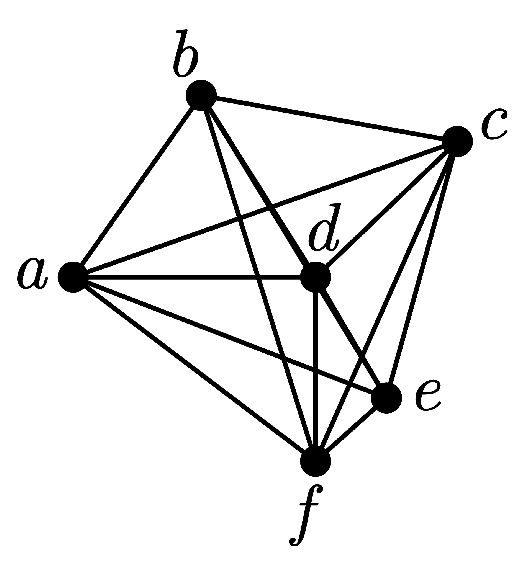
\includegraphics[width=.33\linewidth]{邻域结构-完全图.pdf}}
    \subfloat[邻居结构$\mathcal{N}_1$ \label{subfig:邻域结构1}]{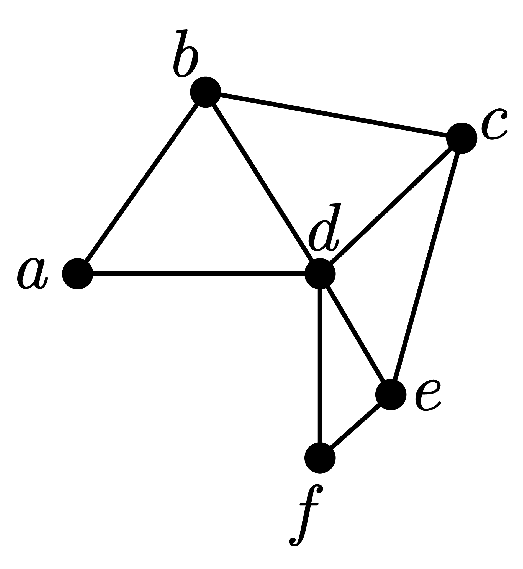
\includegraphics[width=.33\linewidth]{邻域结构-N1.pdf}}
    \subfloat[邻居结构$\mathcal{N}_2$ \label{subfig:邻域结构2}]{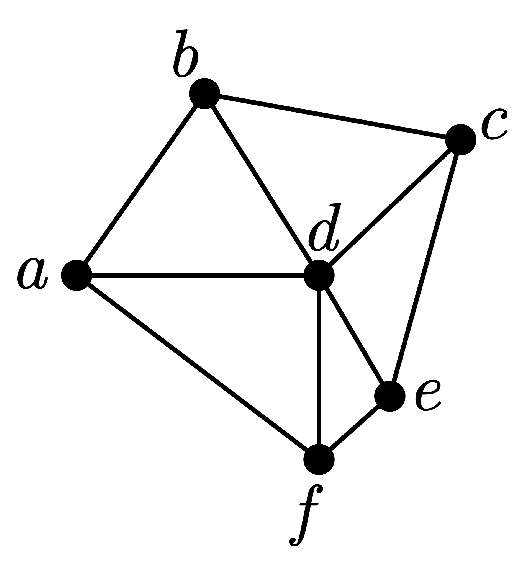
\includegraphics[width=.33\linewidth]{邻域结构-N2.pdf}}
    \caption[邻域结构示意图]{邻域结构示意图}
    \label{fig:邻域结构示意图}
\end{figure}
\begin{figure}[htb]
    \ContinuedFloat
    \subfloat[局部最优解$s^* \in \mathcal{N}_1 \in \mathcal{G}$ \label{subfig:邻域结构1-局部最优解}]{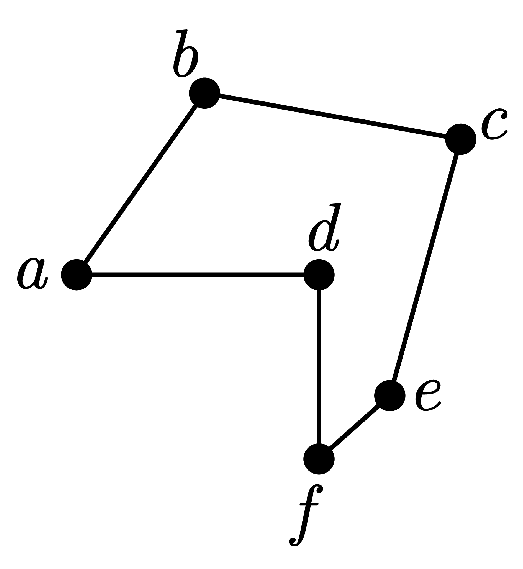
\includegraphics[width=.33\linewidth]{邻域结构-N1-Tour.pdf}}
    \subfloat[全局最优解$s^* \in \mathcal{N}_2 \in \mathcal{G}$ \label{subfig:邻域结构2-全局最优解}]{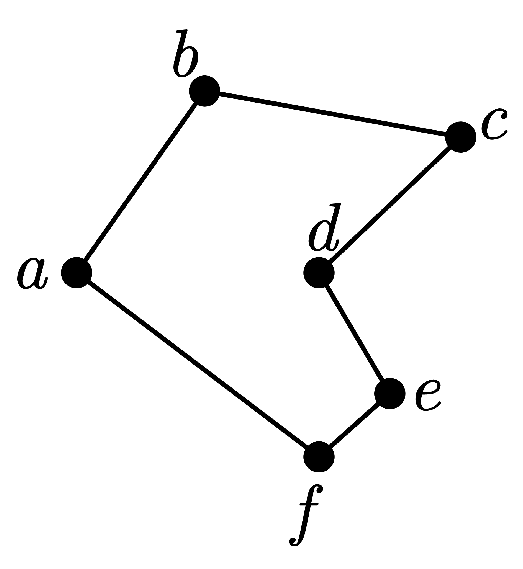
\includegraphics[width=.33\linewidth]{邻域结构-N2-Tour-Opt.pdf}}
    \caption[]{邻域结构示意图(续)}
\end{figure}
\par
如\autoref{fig:邻域结构示意图}~所示,给定一个TSP问题$\mathcal{P}$和问题$\mathcal{P}$的全连接图$\mathcal{G}$,由\autoref{def:邻域结构}~可知,当每个顶点的候选集由剩余所有顶点组成时,那么问题$\mathcal{P}$的邻域结构就是$\mathcal{G}$。在\autoref{fig:邻域结构示意图}~中,\autoref{subfig:全连接图}~就是一个全连接图。由算法~\ref{alg:局部搜索算法框架}~可知,当邻域结构是全连接图时,这使得算法需要搜索整个搜索空间,显然不符合题意。因此,需要对邻域结构进行定制。如\autoref{subfig:邻域结构1}~所示,虽然\autoref{subfig:邻域结构1}~的邻域结构足够的小,但是,它并没有将\autoref{subfig:邻域结构2-全局最优解}~所示的最优路径中的所有边(如边$af$)都包含进去,当算法使用这个邻域结构,不用其他策略时,无论如何也不能搜索到最优解(只能搜索到局部最优解,如\autoref{subfig:邻域结构1-局部最优解})。所以,设计的邻域结构(如\autoref{subfig:邻域结构2})不仅要小,还需要保证足够的质量,以确保算法能够搜索到满意的解。
% 整图
% \begin{figure}[t]
%     \subfloat[全连接图$\mathcal{G}$ \label{subfig:全连接图}]{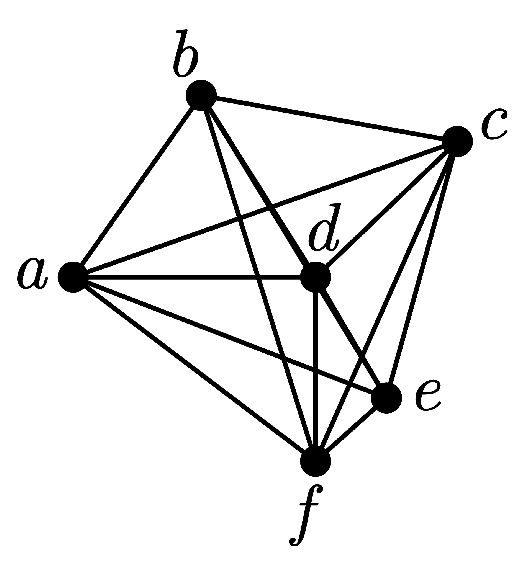
\includegraphics[width=.33\linewidth]{邻域结构-完全图.pdf}}
%     \subfloat[邻居结构$\mathcal{N}_1$ \label{subfig:邻域结构1}]{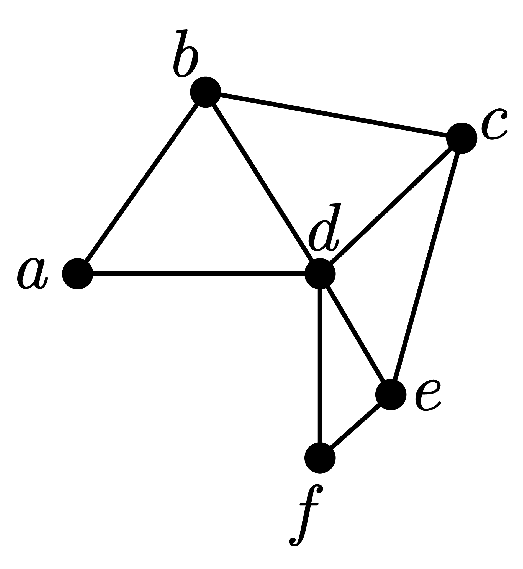
\includegraphics[width=.33\linewidth]{邻域结构-N1.pdf}}
%     \subfloat[邻居结构$\mathcal{N}_2$ \label{subfig:邻域结构2}]{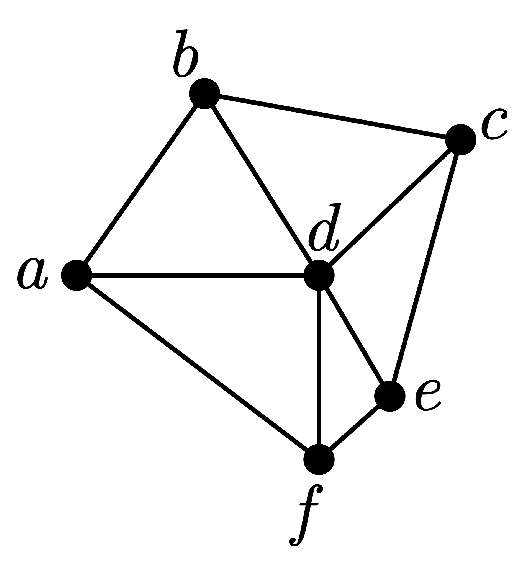
\includegraphics[width=.33\linewidth]{邻域结构-N2.pdf}} \\
%     \subfloat[局部最优解$s^* \in \mathcal{N}_1 \in \mathcal{G}$ \label{subfig:邻域结构1-局部最优解}]{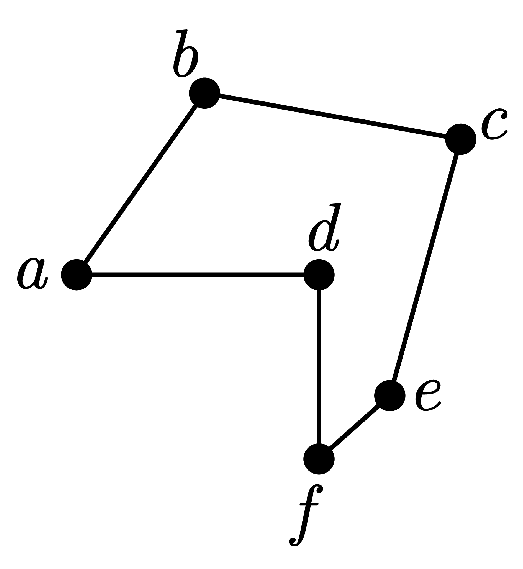
\includegraphics[width=.33\linewidth]{邻域结构-N1-Tour.pdf}}
%     \subfloat[全局最优解$s^* \in \mathcal{N}_2 \in \mathcal{G}$ \label{subfig:邻域结构2-局部最优解}]{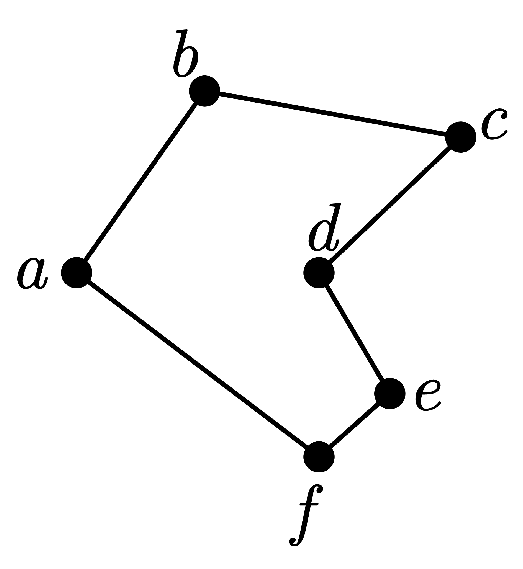
\includegraphics[width=.33\linewidth]{邻域结构-N2-Tour-Opt.pdf}}
%     \caption[邻域结构示意图]{邻域结构示意图}
%     \label{fig:邻域结构示意图}
% \end{figure}

\subsection{邻域动作}
\label{subsec:背景介绍:局部搜索:邻域动作}
由\autoref{def:邻域动作和邻域}~可知,邻域动作是一个函数,通过这个函数,算法能够在当前解的邻域中,生成对应的邻居解集合。由章节~\ref{subsec:背景介绍:多目标组合优化算法:进化算法}~可知,遗传操作(交叉、变异算子)是进化算法中最重要的组件之一,它的作用就是产生新个体。又因为多目标组合优化问题的决策空间是离散且巨大的,这导致交叉、变异等算子生成新个体的效率和质量都达不到要求。因此,将邻域动作作为进化算法的一部分,替代遗传操作在算法中的功能,以局部搜索的思想来产生优质的子代个体。
\par
在组合优化问题中,邻域动作的规则不仅与问题的解的编码形式相关,更是在邻域结构的基础上来进行搜索产生新解的。因此,为保证与邻域的一致性,统一使用TSP和MOTSP。对于TSP问题,其解的编码形式为一个所有顶点组成的序列路径。针对序列路径,产生新个体的方式有很多。比如,有一序列路径$s = <v_1, v_2, v_3, v_4, v_5>$,任意交换两个顶点($v_2, v_3$)的位置\cite{borges1998basis}~,这样就在$s$的基础上,产生了一个$s$的邻居解$s' = <v_1, v_3, v_2, v_4, v_5>$。其中“交换两个顶点”这个动作就是邻域动作。
\par
\autoref{fig:k-opt示意图}~是一种名为k-opt的邻域动作规则\cite{helsgaun2006effective}~,其中k代表要交换的边数,k越大,代表新个体对原解的改动越大,并且,搜索所有解的判断时间也是k的指数倍。\autoref{subfig:2-opt}~中是2-opt移动示意图,原序列路径为$s=<v_1, v_2, v_4, v_3>$,在经由2-opt后,$s$删除$x_1, x_2$两条边,连接$y_1, y_2$两条边得到$s'=\{ v_1, v_4, v_2, v_3 \}$,相当于将$s$中的$x_1, x_2$两条边替换成$y_1, y_2$两条边,由此生成$s'$。同理,\autoref{subfig:3-opt}~为3-opt,\autoref{subfig:4-opt}~为4-opt。从图中很容易知道,一条序列路径$s$经由k-opt操作后,就是将$s$中的k条边,使用特定的交换策略,替换成不属于原序列路径的不同的k条边,这样就可以产生了$s'$。并且,从图中可以看出,k-opt是在(k-1)-opt的基础上再进行一次换边操作的,在使用k-opt时,我们期望k越大,获得的结果越好,并且对于足够大的k,我们期望序列路径$s$经由k-opt操作得到的$s'$应该是最优的。但是,随着k的增大,测试所有可能交换的边所需的操作次数增长得非常快。并且,我们并不知道给定问题到底需要设置多大的k才能获得可接受的优化结果,这也是使用k-opt算子无法避免的一个缺点。
\begin{figure}[htb]
    \subfloat[2-opt \label{subfig:2-opt}]{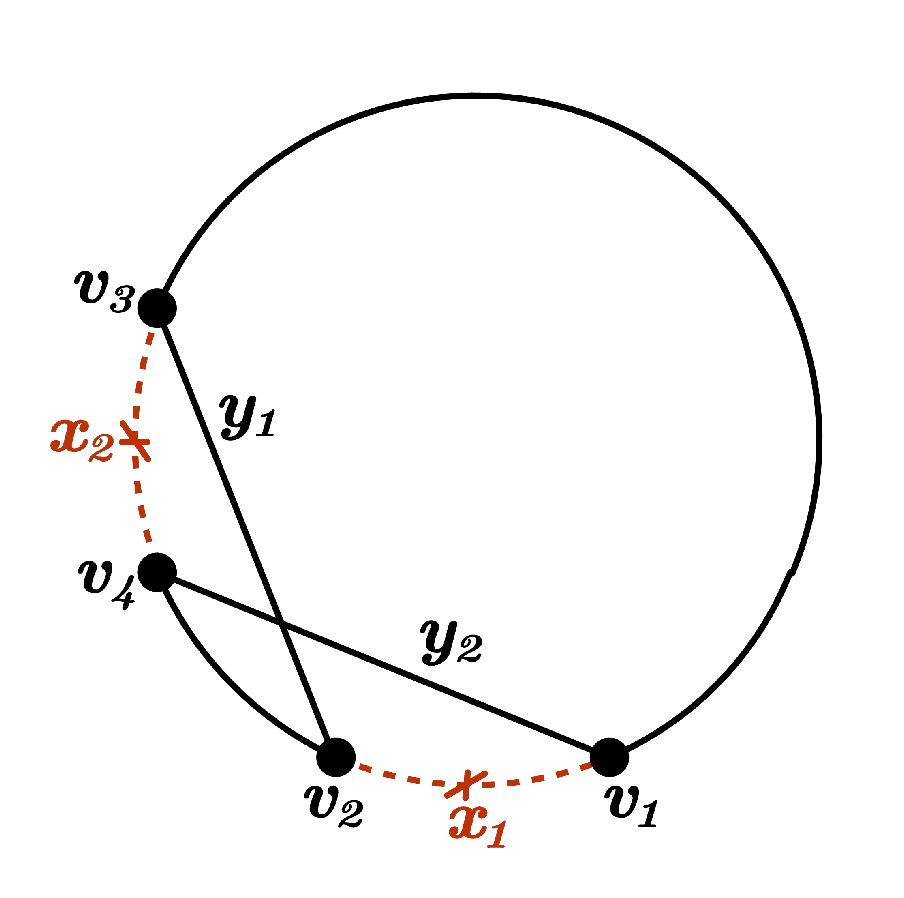
\includegraphics[width=.3\linewidth]{k-opt-2.pdf}}\quad
    \subfloat[3-opt \label{subfig:3-opt}]{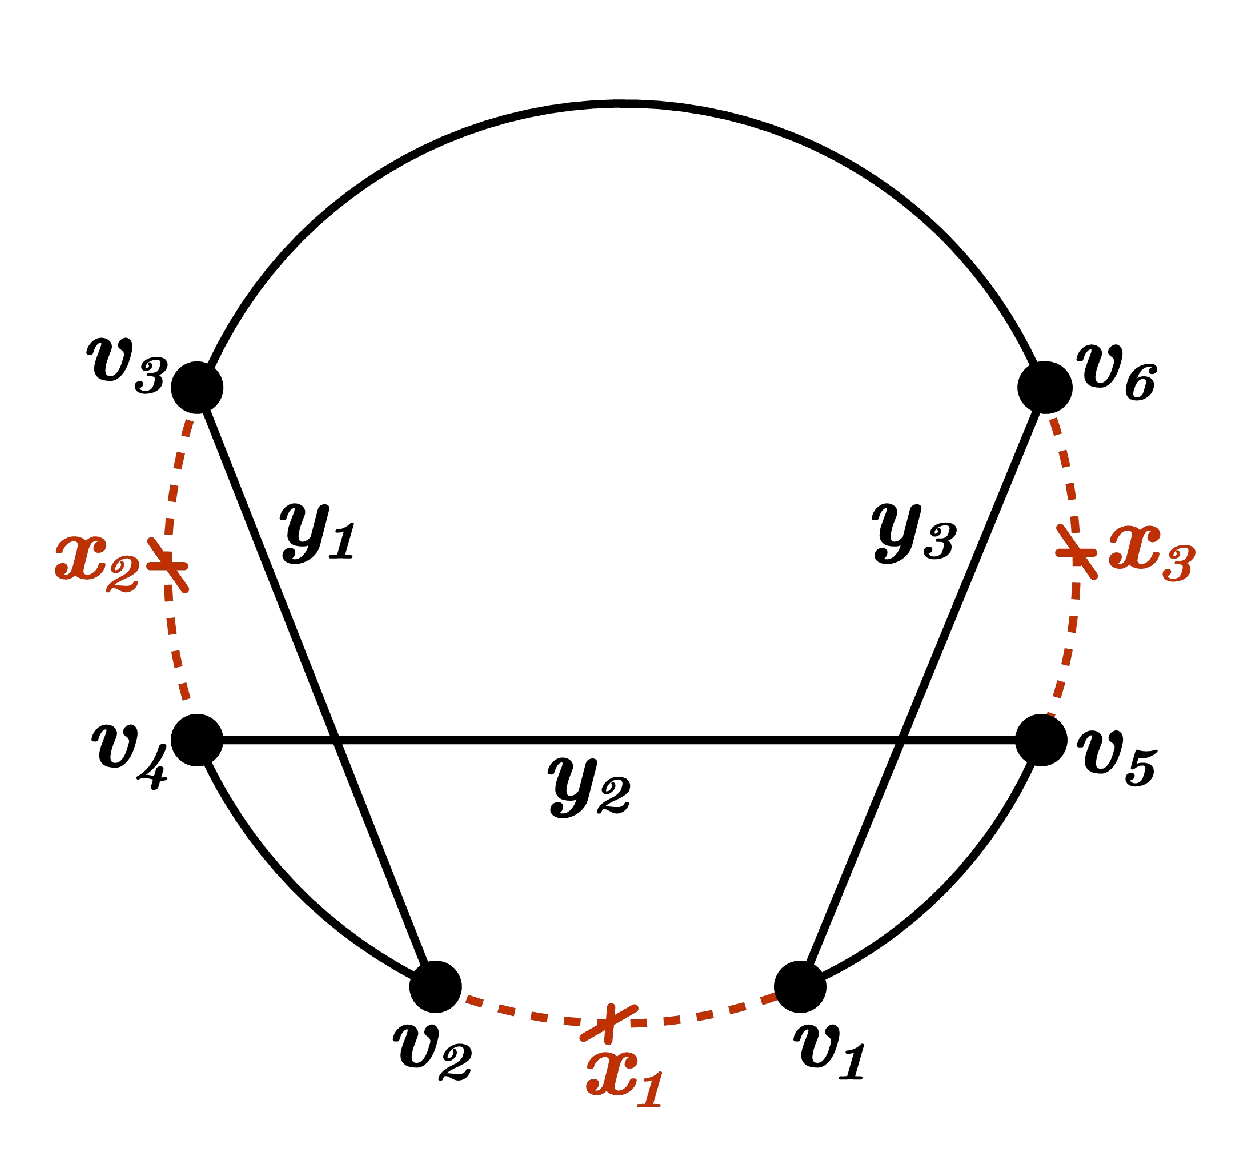
\includegraphics[width=.3\linewidth]{k-opt-3.pdf}}\quad
    \subfloat[4-opt \label{subfig:4-opt}]{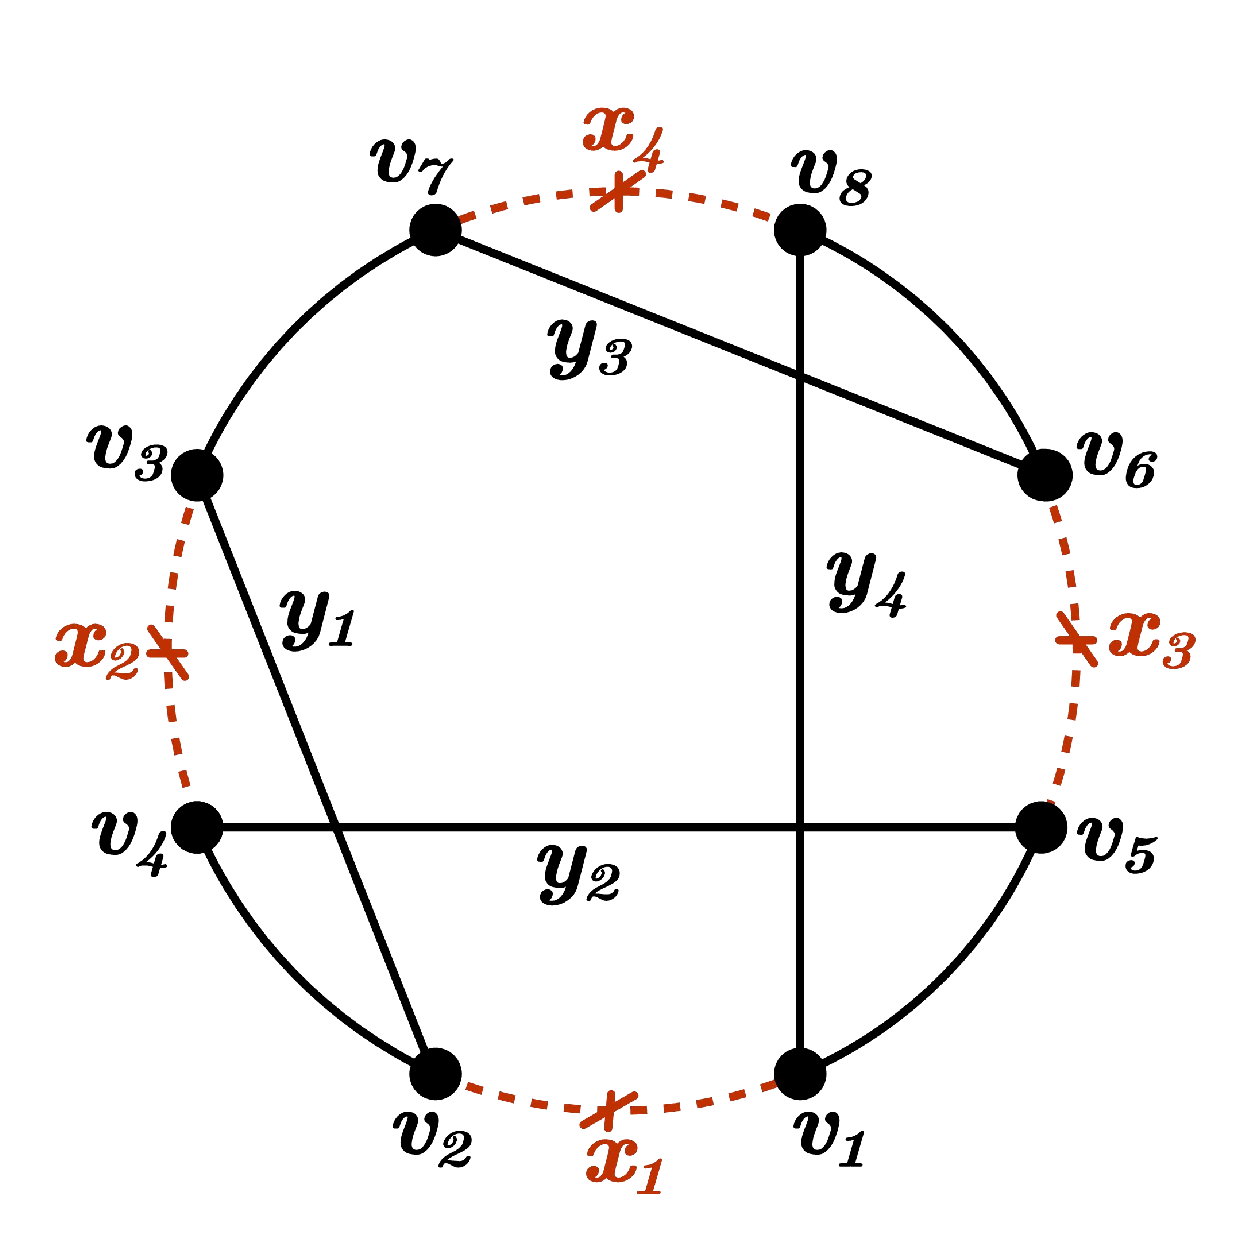
\includegraphics[width=.3\linewidth]{k-opt-4.pdf}}
    \caption[k-opt示意图]{k-opt示意图}
    \label{fig:k-opt示意图}
\end{figure}

% \subsection{Lin-Kernighan算法}
% \label{subsec:背景介绍:局部搜索:Lin-Kernighan算法}
% 针对上一节\ref{subsec:背景介绍:局部搜索:邻域动作}~中,k-opt算法无法确定k值这一缺点,Lin和Kernighan提出了一种补救措施:k-opt算法,k值可变,在执行过程中动态变化。该算法从考虑要交换的一组r=2链接开始,并在每个迭代步骤中决定是否应考虑一组r+1链接。该算法基于以下主要原则:
% \begin{itemize}
%     \item 使用顺序移动;
%     \item 必须选择要在序列中删除的最后一个链接,以便如果序列中没有更多步骤,则可以添加一个链接来结束游览(在每个步骤中,我们都可以停止并进行有效的移动);
%     \item 每个部分的收益总和必须是正的(移动必须是有希望的);
%     \item 删除的链接集和添加的链接集应该分开(一旦链接被删除,就不能再添加;一旦添加了链接,就不能删除;)。
% \end{itemize}

\section{进化迁移优化}
\label{sec:背景介绍:进化迁移优化}
迁移学习使用从源域(Source Domains,SD)中获取的知识来提升不同(但相关)目标域(Target Domains,TD)的学习能力\cite{pan2009survey}。相似地,进化迁移优化(Evolutionary Transfer Optimization,ETO)是一种将EA求解器与知识学习和跨领域信息转移相结合,以实现更好的优化效率和性能的范式。Kay在文中提到\cite{tan2021evolutionary},ETO虽然是一个兴起不久的优化范式,但是它已经在许多优化领域(比如:多任务优化、多目标优化和机器学习等)发挥了重要的作用。
\par
针对多目标优化问题来说,ETO旨在通过学习或迁移解、结构化信息等与问题相关的有用特征,在提高解的质量或搜索速度等方面来提高算法的性能。从算法设计的角度来说,现有的ETO方法可以分为同构(Homogenous)ETO和异构(Heterogeneous)ETO:
\begin{itemize}
    \item \textbf{同构ETO:}共享相同搜索空间的跨问题的知识迁移。
    \item \textbf{异构ETO:}跨具有不同搜索空间的问题之间的知识迁移。
\end{itemize}
此外,同构ETO已通过以不同子问题之间交换PS中解的形式实现跨子问题的知识迁移的方式应用于多目标和超多目标优化问题中\cite{tan2021evolutionary}。如\autoref{fig:跨问题知识迁移示意图}~所示,多目标和超多目标优化中的有用知识可以采用非支配解集、代理模型等形式来实现跨问题的知识迁移。如果ETO取得了在有知识迁移的情况下比没有知识迁移更好(更差)的表现,则称为正(负)迁移。
\begin{figure}[htb]
    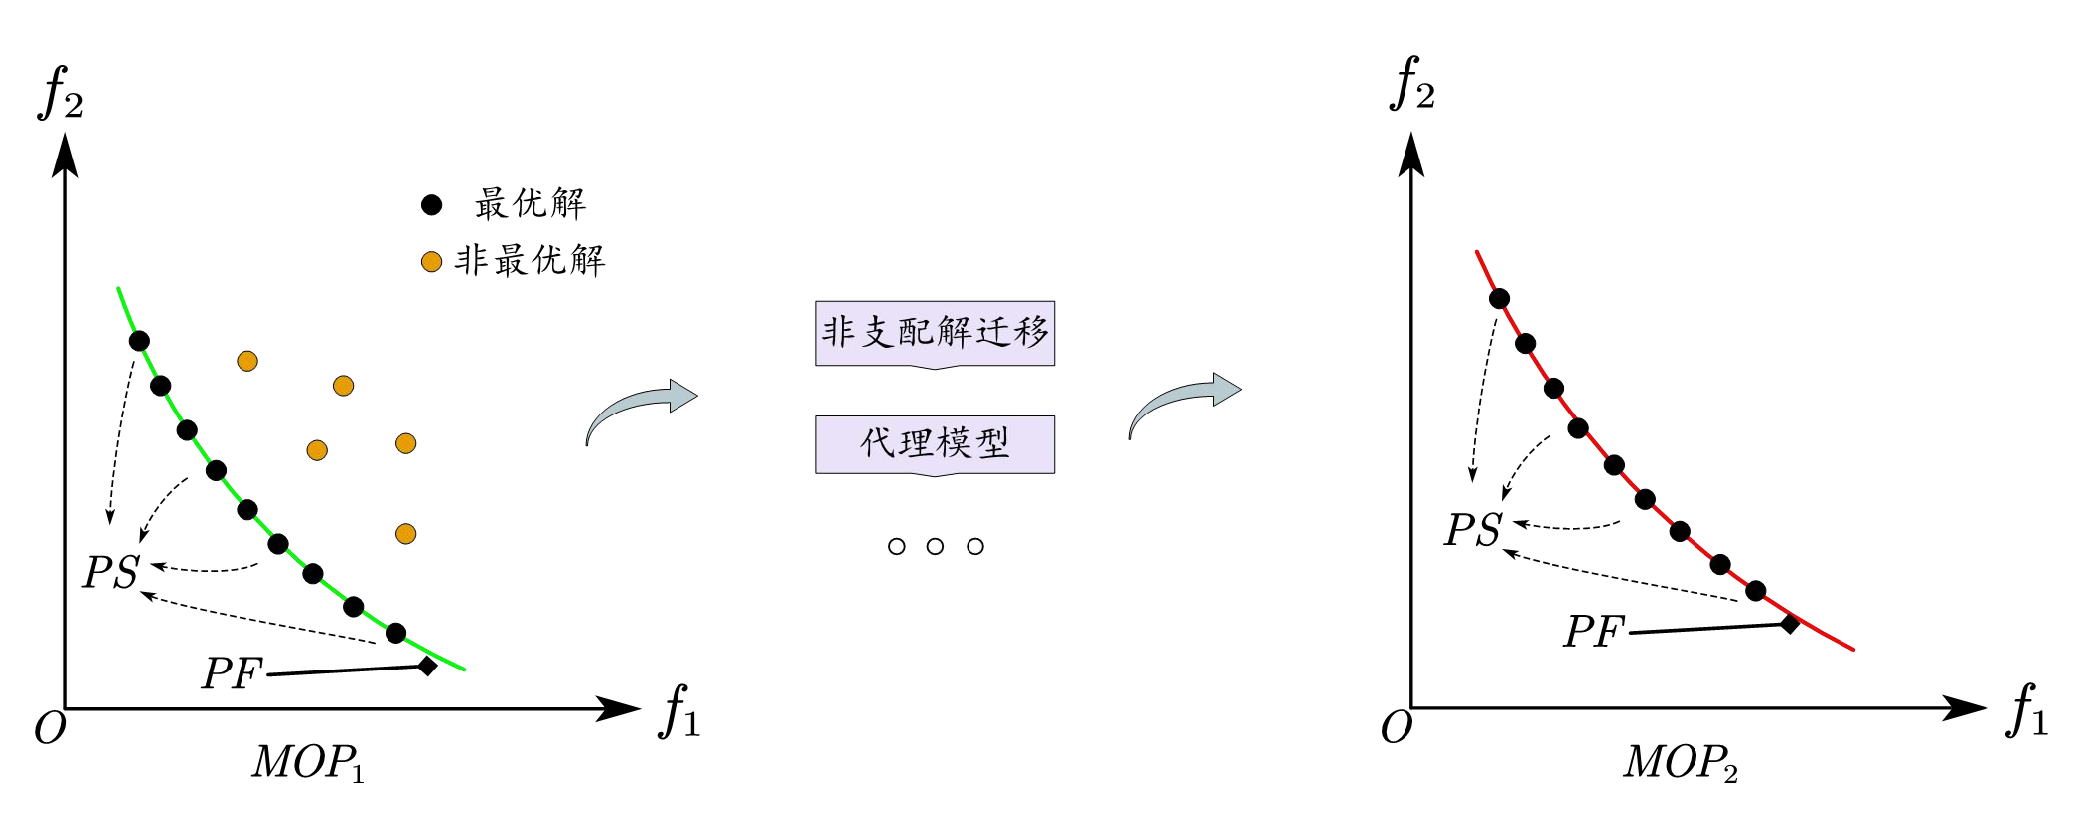
\includegraphics[width=\linewidth]{ETO.pdf}
    \caption[跨问题知识迁移示意图]{跨问题知识迁移示意图}
    \label{fig:跨问题知识迁移示意图}
\end{figure}
\par
直观地说,随着多目标优化问题中目标数量的增加,要迁移的非支配解的数量将急剧增加。因此,与只迁移MOP问题中非支配解的ETO相比,正确地构建源域和目标域中可迁移知识之间的映射关系是我们应该研究的重点。并且我们需要深入分析,在MOP中,什么信息是有用的,以及这些信息如何与跨问题域的多个目标相关连的。这可以更好地了解ETO在多目标和多目标优化中怎样并且在什么时候能够实现正迁移。

\section{性能评价指标}
\label{sec:背景介绍:性能评价指标}
对于一个算法,抛开其本身的复杂性而言,其表现好坏则是通过这个算法所求得相应问题的最终结果的优劣而定。对于CMOPs来说,其最终结果以非支配解集(NDSet,\autoref{def:非支配解集})的形式呈现。所以,一个MOEA的性能通常从两个方面进行评估:
\begin{enumerate}
    \item 群体解集的收敛性:NDSet与真实Pareto前沿(PF)的贴合程度。
    \item 群体解集的多样性:NDSet在空间上分布的均匀程度和广泛程度。
\end{enumerate}
\par
Knowles等人于2006年在文中\cite{knowles2006tutorial}介绍了很多评估NDSet性能的评价指标。例如:超体积度量指标(Hypervolume,HV)\cite{zitzler1999multiobjective}、反向世代距离指标(Inverted Generational Distance,IGD)\cite{czyzzak1998pareto}和集合覆盖度量指标(Set Converage,C-Metric)\cite{zitzler1999multiobjective}等。在本文中,除了需要对MOEA的性能进行评估外,还需要对邻域结构(最优边遗失率指标\cite{helsgaun2018using})和TSP问题的解进行质量评估(距离趋近度指标\cite{helsgaun2018using}),下面将分节详细介绍。

\subsection{超体积度量指标}
\label{subsec:背景介绍:性能评价指标:超体积度量指标}
超体积度量指标HV是一种通过计算参考点与NDSet围成空间的超体积实现对算法综合性能评价的方法,其数学形式如下:
\begin{align}
    \label{eq:HV}
    HV = \mathcal{L} (\bigcup_{i=1}^{|\mathcal{S}|} v_i).
\end{align}
其中,$\mathcal{L}$为Lebesgue测度,$\mathcal{S}$代表NDSet,$| \cdot  \vert $代表集合中元素的个数,$v_i$为非支配个体$s_i \in \mathcal{S}$和参考点$z^*$构成的超体积。
\begin{figure}[htb]
    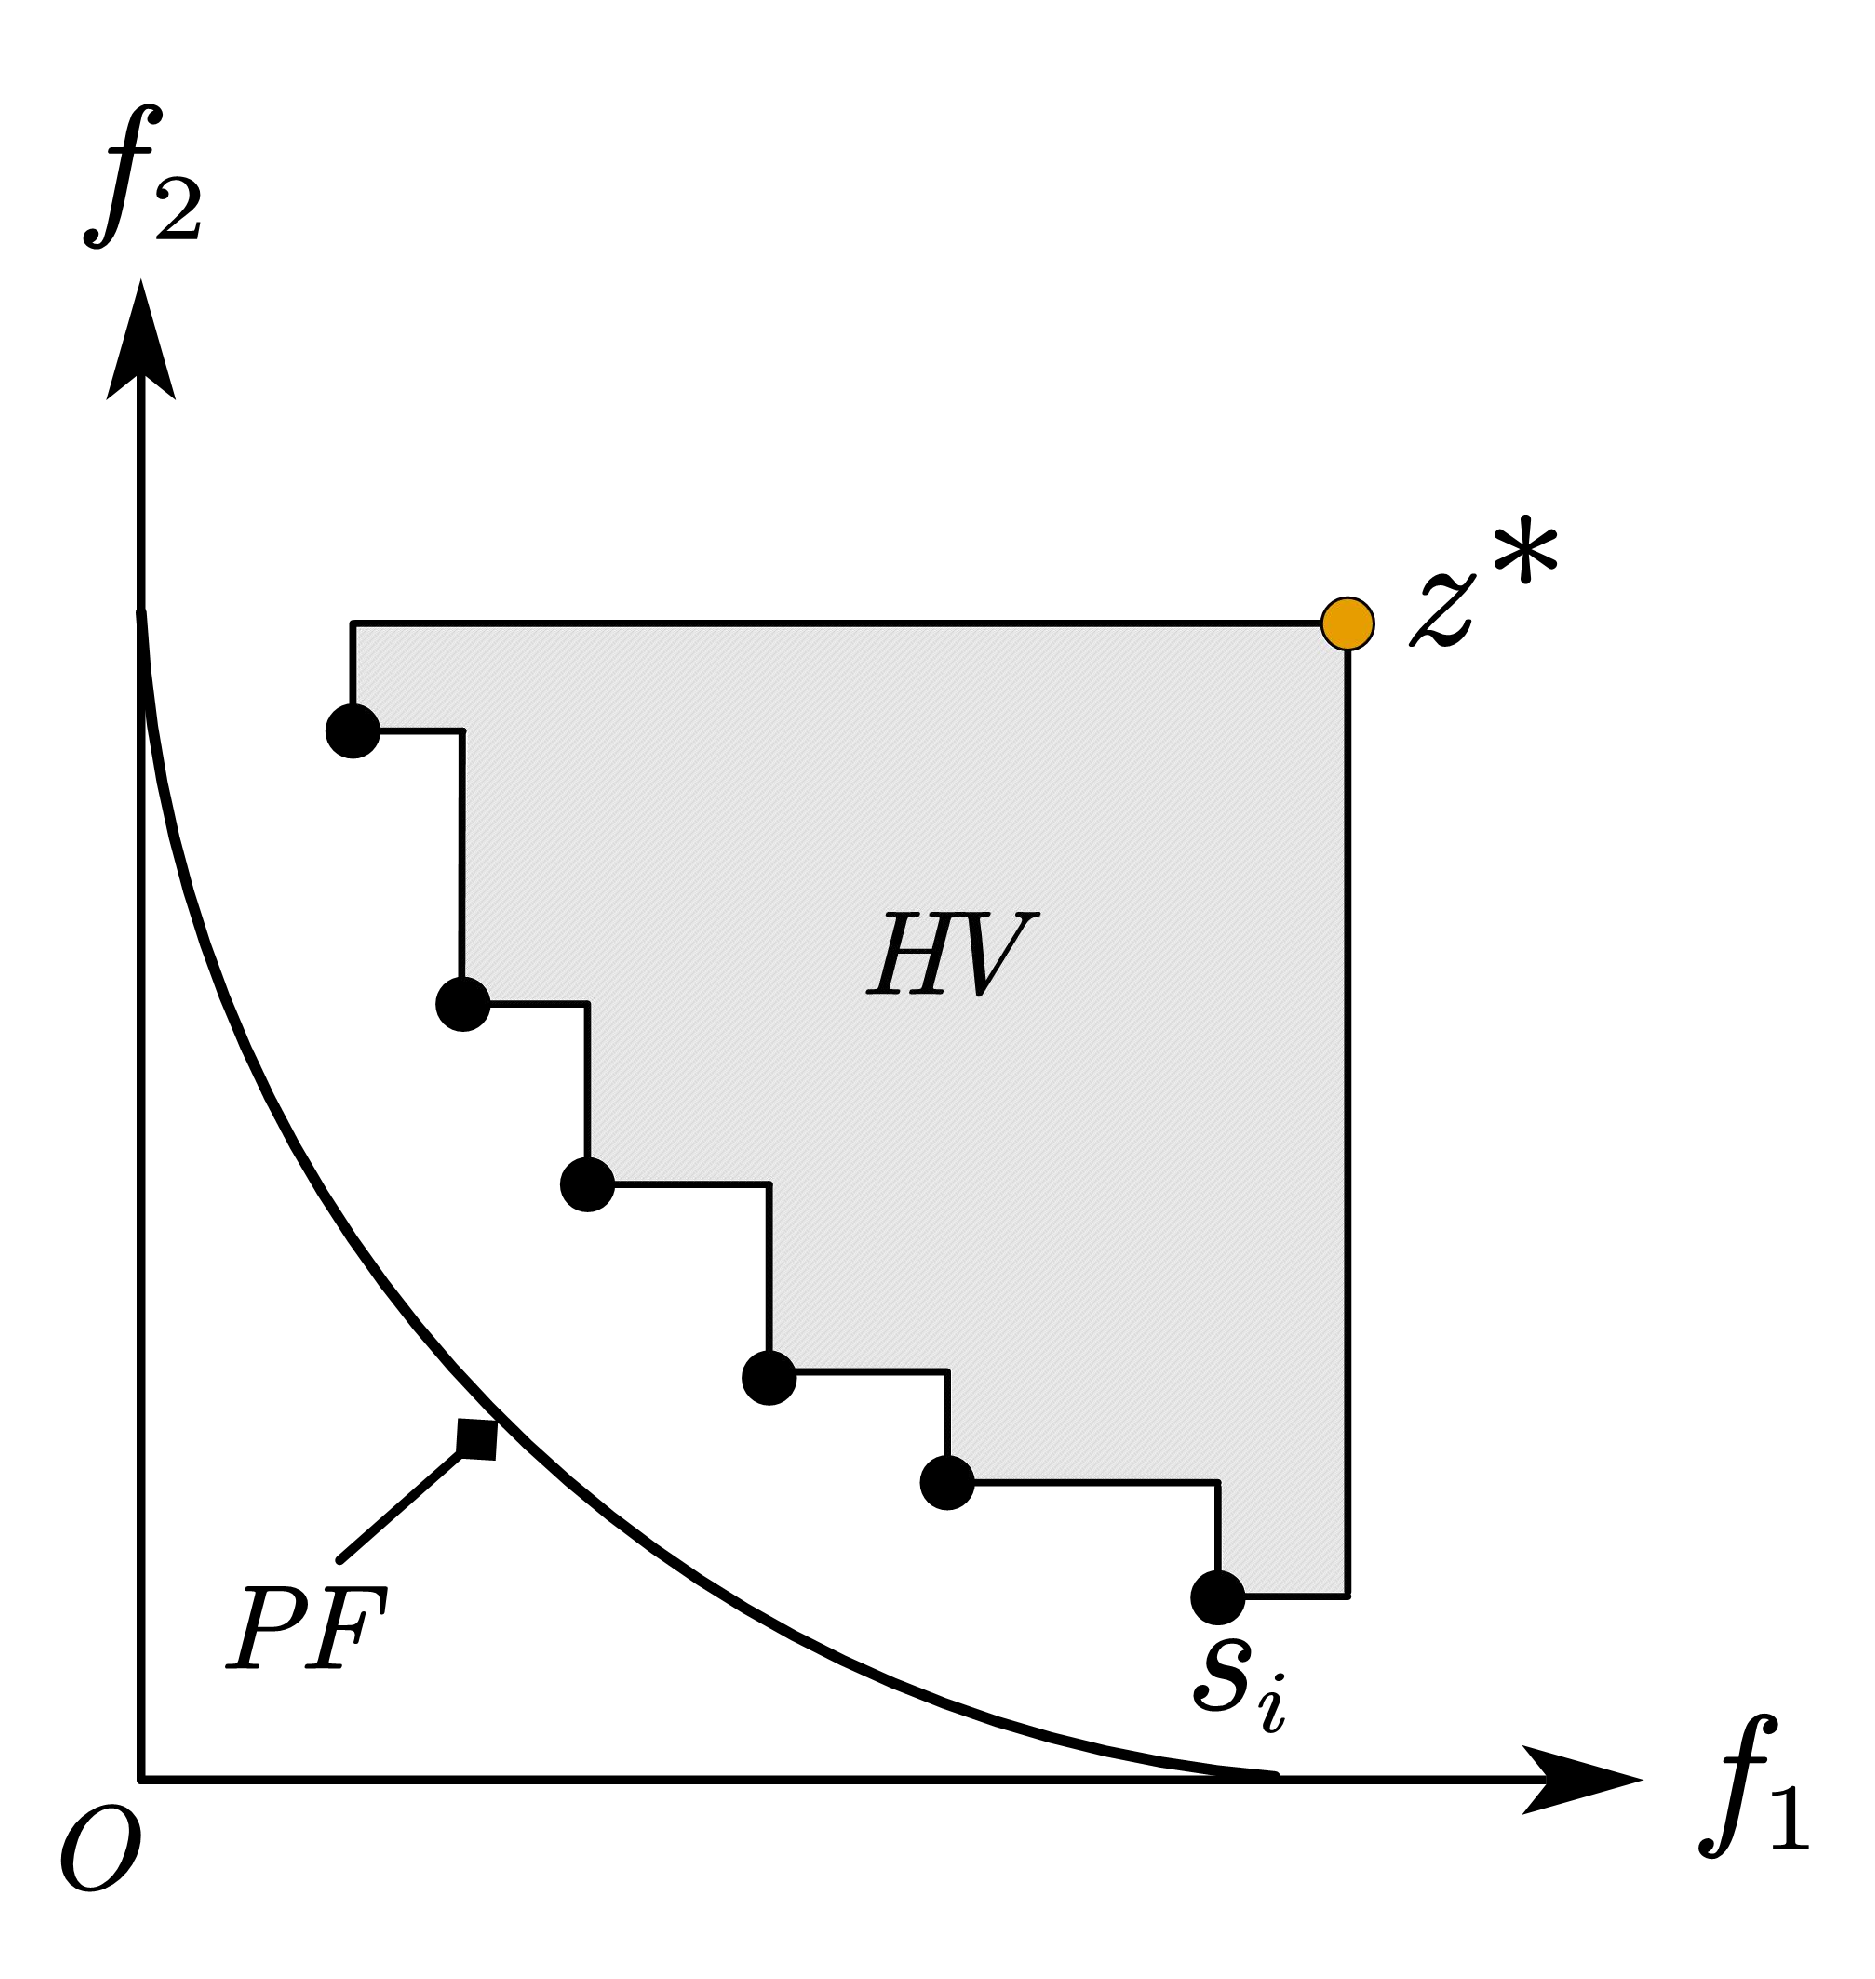
\includegraphics[width=.4\linewidth]{HV.pdf}
    \caption[HV指标示意图]{HV指标示意图}
    \label{fig:HV指标示意图}
\end{figure}
\par
如\autoref{fig:HV指标示意图}~所示是一个二目标问题的非支配解集的超体积度量示意图,其中超体积度量值为NDSet和参考点$z^*$构成的阴影区域的面积。$z^*$的选择方式有多种,常用的有:NDSet每维上的最大值组成的向量和松散形式的最差点\cite{deb2010toward}。从图中容易知道,HV指标值同样遵循Pareto支配(\autoref{def:Pareto支配})原则,以最小化MOP为例,如果个体$s_1 \prec s_2$,则$s_1$的HV度量值一定大于$s_2$,同理,可推广到两个解集之间的支配关系。并且,计算HV指标值时,真实PF不是必需的,所以HV指标具有更好的实用性。但是,计算HV指标的时间复杂度非常大,而且参考点的选择也会影响HV指标的正确性\cite{zheng2007mop}。

\subsection{反向世代距离指标}
\label{subsec:背景介绍:性能评价指标:反向世代距离指标}
反向世代距离指标IGD也是一种兼顾收敛性和多样性的综合评价指标。世代距离是指NDSet中所有个体到Pareto最优解集(PS)的平均距离,而反向世代距离则是PS中的个体到所求NDSet的平均距离。由此,其计算公式可表述如下:
\begin{align}
    \label{eq:IGD}
    IGD = \frac{1}{|PS|} \sum_{\mathbf{x}^* \in PS} \min_{s \in \mathcal{S}} \ \mathit{d}(\mathbf{x}^*, s).
\end{align}
其中,$PS$为Pareto最优解集(真实PF的真子集),$| \cdot  \vert $代表集合中元素的个数,$\mathcal{S}$为非支配解集,$\mathit{d}(\mathbf{x}^*, s)$代表个体$\mathbf{x}^*$与个体$s$的欧几里得距离。IGD值越小,说明算法的综合性能越好。
\begin{figure}[htb]
    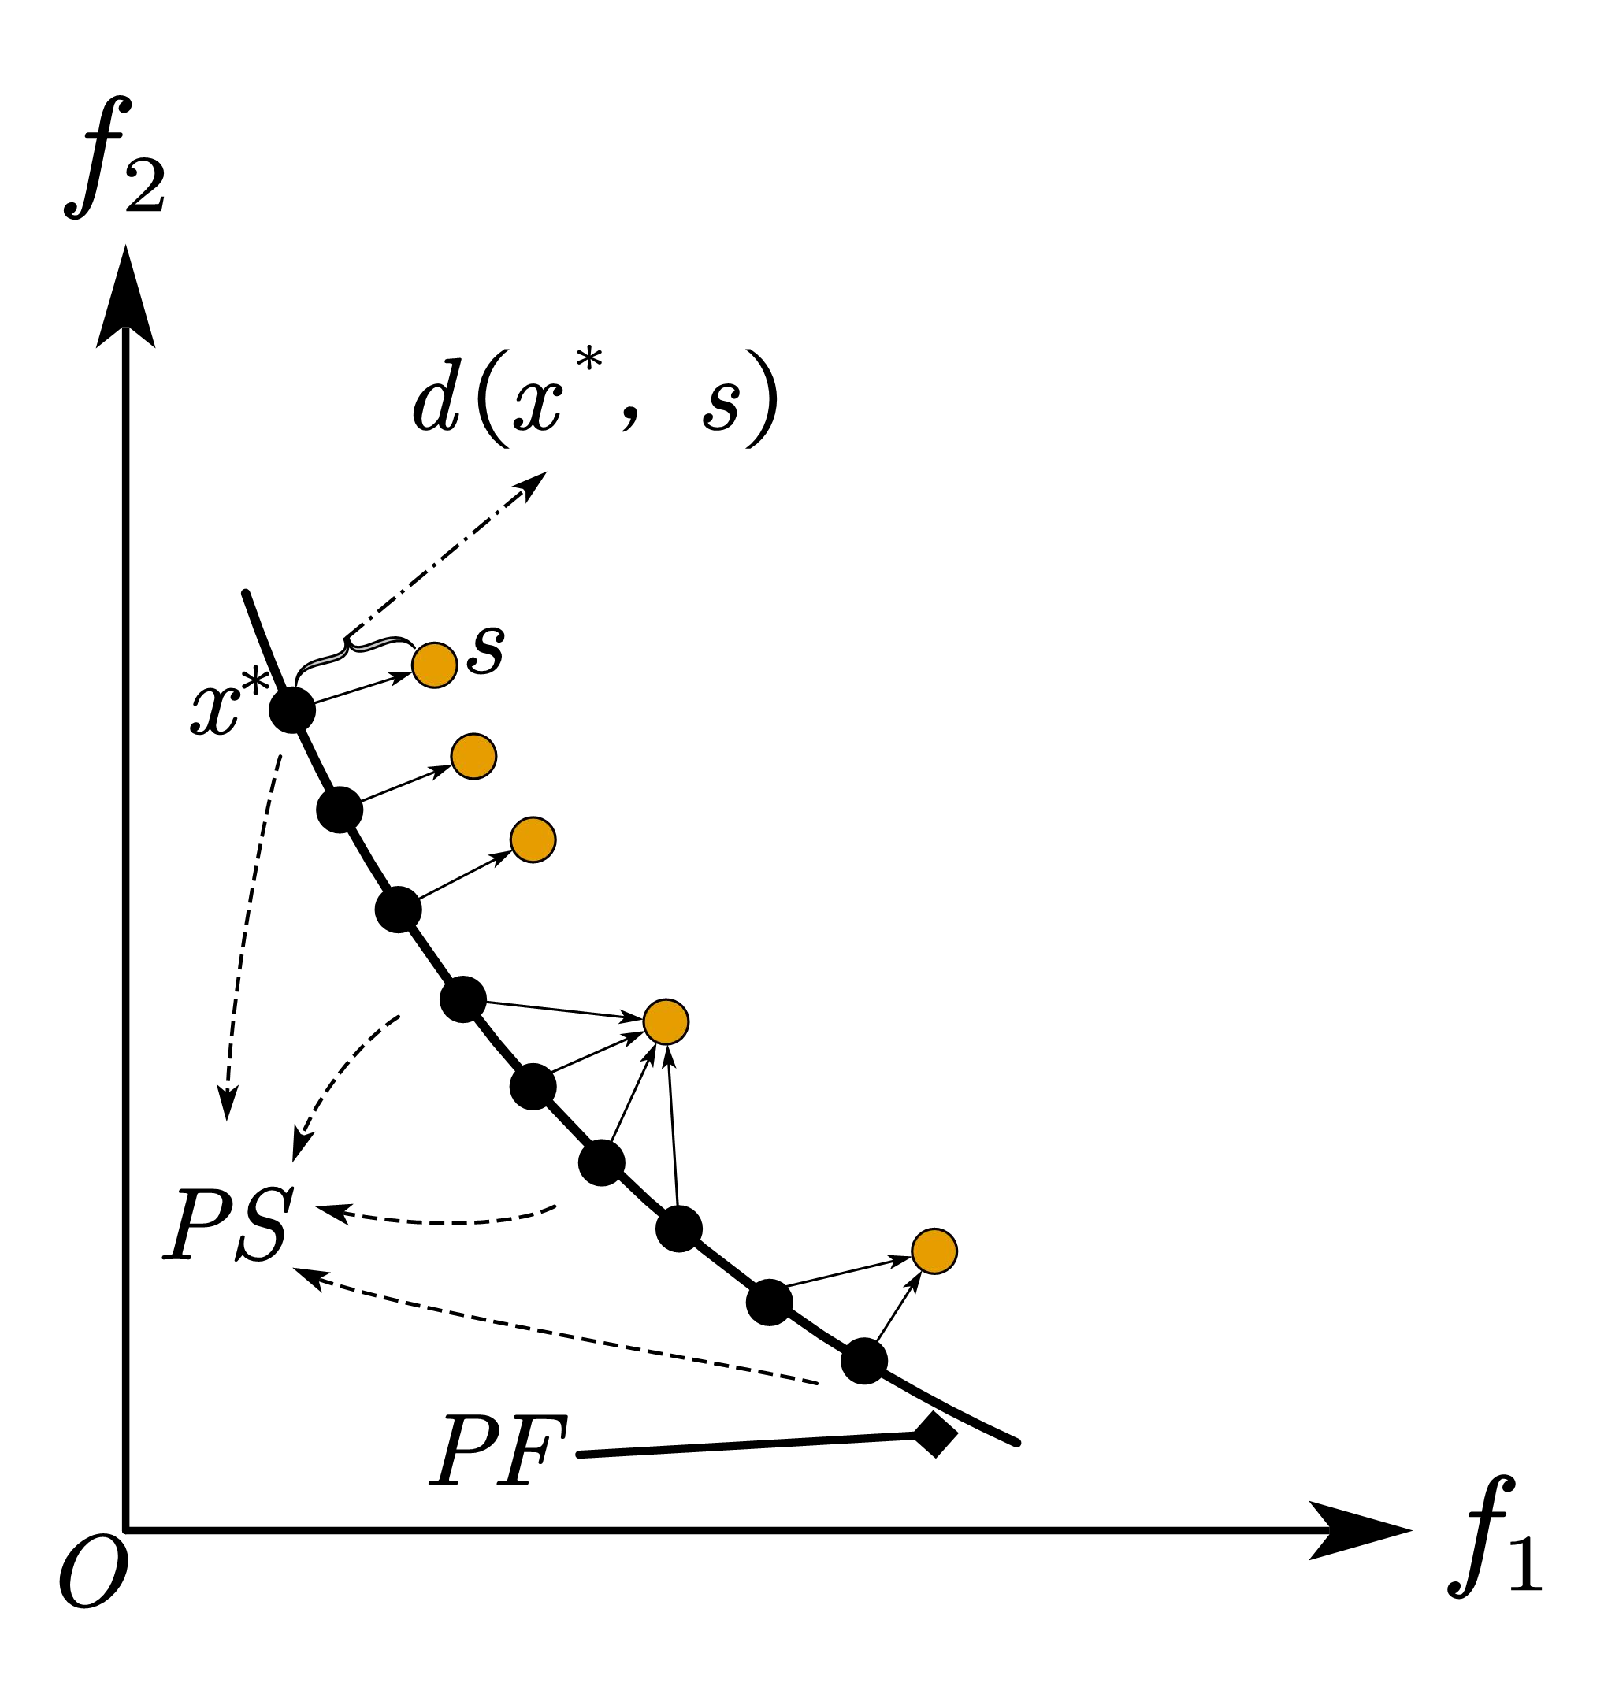
\includegraphics[width=.4\linewidth]{IGD.pdf}
    \caption[IGD指标示意图]{IGD指标示意图}
    \label{fig:IGD指标示意图}
\end{figure}
\par
此外,由\autoref{fig:IGD指标示意图}~可以直观地理解IGD指标对解集的综合性能评价。从图中可以看到,NDSet距离PF的距离远近能够直观地表现收敛性的好坏。同时,可以观察到,当NDSet的分布性不好时,由\autoref{eq:IGD}~计算可得IGD评价值会变大,并且在图中也可以看出,当NDSet分布均匀且广泛时,IGD评价值会很小。因此可以说明IGD评价指标不仅能够反映解集的收敛性,而且能够刻画解集的多样性(广泛且均匀)。但是,IGD指标需要通过真实PF来计算指标值,而现实问题大多都不知道其真实最优解,所以,这也成为其缺陷之一。

\subsection{集合覆盖度量指标}
\label{subsec:背景介绍:性能评价指标:集合覆盖度量指标}
集合覆盖度量指标C-Metric是一种两个解集相对覆盖率比较的方法,其利用解与解互相间的支配关系来判断两个解集之间的收敛性能的优劣。在C-Metric中,设在目标空间中有两个非支配解集$\mathcal{S}_a, \mathcal{S}_b \subseteq \mathcal{S}$,C-Metric则将($\mathcal{S}_a, \mathcal{S}_b$)映射到$[0, 1]$之间,得到$\mathcal{S}_a$与$\mathcal{S}_b$两解集之间的覆盖率,其数学形式如下:
\begin{align}
    \label{eq:C-Metric}
    C(\mathcal{S}_a, \mathcal{S}_b) = \frac{|\{ b \in B \ | \ \exists a \in A, a \prec b \}|}{|\mathcal{S}_b|} \times 100\%.
\end{align}
其中$| \cdot  \vert $代表集合中元素的个数,$C(\mathcal{S}_a, \mathcal{S}_b)$代表$\mathcal{S}_b$中所有能被$\mathcal{S}_a$中的解支配的解的数目占$\mathcal{S}_b$中解数目的百分比。
\par
由上述定义可知,如果$\mathcal{S}_a$中的解都弱支配$\mathcal{S}_b$中的解,那么C-Metric的值等于1,反之为0。一般的,由于$\mathcal{S}_a$和$\mathcal{S}_b$的交集并不为空,所以在评估解集的质量时,需要同时考虑$C(\mathcal{S}_a, \mathcal{S}_b)$和$C(\mathcal{S}_b, \mathcal{S}_a)$。要注意C-Metric方法并不是解集之间的距离上的比较,而是不同解集在支配关系上的相对比较。C-Metric的优点在于计算简单,但是计算复杂度取决于非支配排序算法,当目标数很大时,非支配排序算法的复杂度会很高,会耗费大量时间计算该指标。

\subsection{距离趋近度指标}
\label{subsec:背景介绍:性能评价指标:距离趋近度指标}
距离趋近度指标是一种用来评判单目标解质量的方法。对于最小化优化问题而言,距离趋近度指标利用解的适应值超过已知最优解的适应值的百分比来评判解的质量。假设有解$s$和最优解$s^*$,适应度函数$\varphi$,则其数学形式如下:
\begin{align}
    \label{eq:Gap}
    Gap = \frac{|\varphi (s) - \varphi (s^*)|}{\varphi (s^*)} \times 100\%.
\end{align}
其中$| \cdot  \vert $代表集合中元素的个数,一般地,我们很难知道具体问题的最优解,所以$s^*$一般可以用目前已知最优解来代替。
\par
由\autoref{eq:Gap}~可知,当适应度函数为线性函数时,其适应值就可以表现为解的值,当算法求得的解距离最优解越近,其Gap值就越小,代表该解质量越好。因此,可以利用距离趋近度指标来评估不同解的质量。

\subsection{最优边遗失率指标}
\label{subsec:背景介绍:性能评价指标:最优边遗失率指标}
最优边遗失率指标是一种评估邻域结构质量的方法。对于图优化问题(如TSP、MST)而言,它们的解都是一个序列路径(节点之间可以构成边)构成。所以,最优边遗失率指标计算的是,邻域结构中,缺失的最优边(最优解中的边)的数目占最优解中边的数目的百分比。其数学描述如下:
\begin{align}
    \label{eq:Missing}
    Missing = (1 - \frac{|\{ e \ | \ e \in  \mathcal{E} (s^*) \bigcap \mathcal{E} (\mathcal{N}) \} |}{|\mathcal{E} (s^*)|}) \times 100\%.
\end{align}
其中$| \cdot  \vert $代表集合中元素的个数,$s^*$为最优解(一般用目前已知最优解替代),$\mathcal{N}$为邻域结构,$\mathcal{E} (\cdot)$获取解或者邻域结构中的边。
\par
由\autoref{eq:Missing}~可知,最优边遗失率指标仅能描述邻域结构的质量,并不能表示邻域结构的冗余度。当邻域结构是完全图(包含整个问题)时,那么它一定包含最优解中的所有边,Missing值为0,但这并不代表这个邻域结构是我们所期望的。所以,在用最优边遗失率指标对邻域结构进行评估时,应该建立在多个被评估的邻域结构拥有同样的稀疏度(出入度)的基础上。

\section{测试问题}
\label{sec:背景介绍:测试问题}
在本节中,将会介绍适用于本文的测试问题。由于本文提出了一种针对旅行商问题(Traveling Salesman Problem,TSP)的邻域结构生成的方法,为后续的基于邻域结构迁移的多目标进化算法提供一个可用于迁移的知识模型,所以,在本文将会用到单目标的TSP问题作为邻域结构生成的测试用例。又因为,邻域结构具有专属性(一种结构模型可能只适用于专属的问题),所以本文将使用多目标旅行商问题(Multi-Objective Traveling Salesman Problem,MOTSP)作为基于邻域结构迁移的多目标进化算法的测试用例。同时,在最后还会介绍多目标最小生成树问题( Multi-criteria Minimum Spanning Tree,MCMST),该问题具有和MOTSP类似的邻域结构,可以使用MOTSP的邻域结构尝试解决MCMST。本文提出的是解决具有图邻域结构组合优化问题的算法框架,有兴趣的读者可以尝试用该框架解决其他类型的多目标组合优化问题,介绍MCMST仅为读者提供思路启发。

\subsection{TSP}
\label{subsec:背景介绍:测试问题:TSP}
旅行商问题(TSP)是一种NP难的组合优化问题\cite{johnson1990traveling,baraglia2001hybrid,johnson2007experimental},最早于1959年Dantzig等人提出,并且在最优化领域中得到了深入的研究,同时许多优化方法都是用TSP作为一个测试基准。经典的TSP可以描述为:一个商品推销员想要去若干个城市推销商品,该推销员从其中一个城市出发,不重复的经过所有城市,最后回到出发地。推销员应该制定怎样的旅行路线,使得总行程最短。
\par
从图论的角度而言,TSP实质是在一个带权完全无向图中,找一个权值最小的哈密顿回路。该问题可抽象如下:给定一个完全图$\mathcal{G}=(V,E)$,其中$V = \{ v_1, \cdots, v_n \}$为包含$n$个元素的点集,$E = \{ e_{i,j} = (v_i,v_j) \ | \ v_i,v_j \in V, i \not = j \}$为包含$n^2-n$个元素的边集,寻找一条路径序列$\mathcal{T} = <t_1, \cdots, t_n>, t_i \in V $(所有点都被访问且仅访问一次)使得权重总和$f(\mathcal{T})$最小:
\begin{align}
    \label{eq:TSP}
    minimize \quad f(\mathcal{T}) = d(t_n,t_1) + \sum_{i=1}^{n-1} d(t_i,t_{i+1}).
\end{align}
其中,$d(v_i, v_j)$为边$e_{i,j}$的距离(权重)。

\subsection{MOTSP}
\label{subsec:背景介绍:测试问题:MOTSP}
多目标旅行商问题(MOTSP)相当于是TSP的一个扩展。TSP中,边权仅考虑了距离,所以在计算的时候只需要求总距离最短的路径序列。对于MOTSP而言,边权不仅只考虑距离,还会考虑旅行时间、费用等多种类型的权重,每多一种权重就相当于问题多了一个目标。所以,在求解MOTSP时,我们需要对多个权重(目标)进行权衡,从而给出一组非支配解作为MOTSP的解决方案。与TSP类似,MOTSP同样是选择一条路径序列$\mathcal{T} = <t_1, \cdots, t_n>, t_i \in V $,使得各目标权重总和最小,其数学描述如下:
\begin{align}
    \label{eq:MOTSP}
    minimize \quad f_k(\mathcal{T}) & = d_k(t_n,t_1) + \sum_{i=1}^{n-1} d_k(t_i,t_{i+1}), \\
    k & \in \{1, \cdots, m\}. \notag
\end{align}
其中,$d_k(v_i, v_j)$为边$e_{i,j}$第$k$个目标上的权重。
% MOTSP因其易于理解、模型简单等特点,被众多多目标组合优化算法用作基准测试问题\cite{cheng2012multi,shim2012hybridxia2017reference}。

\subsection{MCMST}
\label{subsec:背景介绍:测试问题:MCMST}
最小生成树(Minimum Spanning Tree,MST)问题是一个经典的组合优化问题,其目标是构造一个带全图的最小权值总和的生成树。设有一个带权无向图$\mathcal{G}=(V,E,W)$,其中$V = \{ v_1, \cdots, v_n \}$为点集,$E = \{ e_{i,j} = (v_i,v_j) \ | \ v_i,v_j \in V, i \not = j \}$为边集,$W = \{ w_{i,j} \ | \ e_{i,j} \in E, i \not = j \}$为边权集,寻找一个包含所有点的树$\mathcal{T} = (V, E_{\mathcal{T}}, W_\mathcal{T}), E_{\mathcal{T}} \subset E,W_\mathcal{T} \subset W$,使得$W_\mathcal{T}$最小,则称$\mathcal{T}$为图$\mathcal{G}$的最小生成树。
\par
与MOTSP类似,当考虑多种类型的权重时,该问题就是一个多目标最小生成树(Multi-criteria Minimum Spanning Tree,MCMST)问题。所以,MCMST的解同样为一组非支配解,其中每个解都是一个最小生成树的边集$E_{\mathcal{T}}$,则其数学描述如下:
\begin{align}
    \label{eq:MCMST}
    minimize \quad f_k(\mathcal{T}) & = \sum_{e_{i,j} \in E_{\mathcal{T}}} w_{i,j}^k, \\
    k & \in \{1, \cdots, m\}. \notag
\end{align}
其中,$w_{i,j}^k$为边$e_{i,j}$第$k$个目标上的权重。容易知道解$\mathcal{T}$中包含$n$个顶点,$n-1$条边。

\section{本章小结}
\label{sec:背景介绍:本章小结}
本章的主要目的是为后续章节提供一定的基础理论支撑。本章在一开始就介绍了多目标优化问题的定义及相关概念,并由此对多目标进化的基础算法进行了简要的介绍,同时详细介绍了基于分解的多目标进化算法。然后针对进化算法在组合优化中遗传算子效率的问题,引出了在基于分解的多目标进化算法中使用局部搜索来对多目标组合优化问题进行优化的思想。接着介绍了与其他领域相结合的进化迁移优化相关概念。最后,介绍了一些性能评价指标和经典的测试问题。